% This file is modified by Frans Oliehoek <faolieho@science.uva.nl>
% on 2005/12/18. (original file name: conference-ornate-20min.en.tex)

\documentclass[9pt, CJK]{beamer}

% This file is a solution template for:
% - Talk at a conference/colloquium.
% - Talk length is about 20min.
% - Style is ornate.



% Copyright 2004 by Till Tantau <tantau@users.sourceforge.net>.
%
% In principle, this file can be redistributed and/or modified under
% the terms of the GNU Public License, version 2.
%
% However, this file is supposed to be a template to be modified
% for your own needs. For this reason, if you use this file as a
% template and not specifically distribute it as part of a another
% package/program, I grant the extra permission to freely copy and
% modify this file as you see fit and even to delete this copyright
% notice. 

\mode<presentation>
{
	%\usetheme{IAS_sidebar} 	% only a simple left side bar, frame-title box varies in size when using subtitles for frames.
	%\usetheme{IAS_sidebar2_10pt} 	% only a simple side bar, the frame-title box has a fixed size to exactly fit a title and subtitle. For usage with 10pt font, i.e.: \documentclass[10pt]{beamer}
	%\usetheme{IAS_sidebar2_11pt} 	% As above only changed to fit 11pt fonts.
	%\usetheme{IAS_sidebar2_12pt} 	% As above only changed to fit 12pt fonts.
	\usetheme{IAS_sidebarNav} 	% An IAS side bar with navigation
	%\usetheme{IAS_topNav}		% Only top navigation with IAS colors
	%\usetheme{IAS_topNav_bottomAuthorTitle}	%Top navigation and author/title in the bottom with IAS colors
	%\usetheme{IAS_topNav_leftIASbar_10pt}	% both top navigation and the IAS sidebar, the frame-title box has a fixed size to exactly fit a title and subtitle. For usage with 10pt font, i.e.: \documentclass[10pt,english
	%\usetheme{IAS_topNav_leftIASbar_11pt}	% As above only changed to fit 11pt fonts.
	%\usetheme{IAS_topNav_leftIASbar_12pt}	% As above only changed to fit 12pt fonts.
	\setbeamercovered{transparent}
	%   % or whatever (possibly just delete it)
}


% to remove the navigation symbols:
%\setbeamertemplate{navigation symbols}{}

\usepackage[english]{babel}

% or whatever

\usepackage[utf8]{inputenc}
% or whatever

\usepackage{times}
\usepackage[T1]{fontenc}
% Or whatever. Note that the encoding and the font should match. If T1
% does not look nice, try deleting the line with the fontenc.
\usepackage{colortbl}
\definecolor{mycyan}{cmyk}{.3,0,0,0}
\usepackage{booktabs, multirow, enumerate}
\usepackage{ctex}
\usepackage{setspace}
%\usepackage{CJK,CJKnumb}

\usepackage{ulem}


\usepackage{subfigure}
\usepackage{graphicx}
\usepackage{color, soul} 
 \usepackage{amsmath} 
 \usepackage{amsthm}
 \usepackage{mathptmx}

% Delete this, if you do not want the table of contents to pop up at
% the beginning of each subsection:
\AtBeginSection[]
{
	\begin{frame}<beamer>
		\frametitle{目录}
		\tableofcontents[currentsection]
	\end{frame}
}
% If you wish to uncover everything in a step-wise fashion, uncomment
% the following command: 

%\beamerdefaultoverlayspecification{<+->}
\newcommand{\tabincell}[2]{\begin{tabular}{@{}#1@{}}#2\end{tabular}}  %表格自动换行




% If you have a file called "university-logo-filename.xxx", where xxx
% is a graphic format that can be processed by latex or pdflatex,
% resp., then you can add a logo as follows:
% \pgfdeclareimage[height=0.5cm]{university-logo}{university-logo-filename}
% \logo{\pgfuseimage{university-logo}}
\graphicspath{{figures/}}
%\pgfdeclaremask{mymask}{figures/thu_logo2-mask}
%\pgfdeclareimage[width=0.45\textwidth,mask=mymask]{image2}{pictures/wai1}
\pgfdeclareimage[width=1.6cm,height=1.0cm]{institution-logo}{figures/gzulogo}
\logo{\pgfuseimage{institution-logo}}

%\includeonlyframes{mine}
\begin{document}
	\renewcommand{\figurename}{图}
	\renewcommand{\tablename}{表}
	\setulcolor{red} 
	
	\newcommand{\CTL}{\textrm{CTL}}
	\newcommand{\CTLsnf}{{\textsc{SNF}_{\textsc{ctl}}^g}}
	\newcommand{\ResC}{{\textsc{R}_{\textsc{ctl}}^{\succ, S}}}
	\newcommand{\CTLforget}{{\textsc{F}_{\textsc{ctl}}}}
	\newcommand{\Ind}{\textrm{Ind}}
	\newcommand{\Pos}{\textit{Pos}}
	\newcommand{\Neg}{\textit{Neg}}
	\newcommand\wrt{{\it w.r.t.}}
	\newcommand{\Hm} {{\cal M}}
	\newcommand{\Hw} {{\cal W}}
	\newcommand{\Hr} {{\cal R}}
	\newcommand{\Hb} {{\cal B}}
	\newcommand{\Ha} {{\cal A}}
	\newcommand{\Mod}{\textit{Mod}}
	
	\newcommand{\rto}{\rightarrow}
	\newcommand{\Muforget}{{\textsc{F}_{\textsc{$\mu$}}}}
	\newcommand{\lto}{\leftarrow}
	\newcommand{\lrto}{\leftrightarrow}
	\newcommand{\Rto}{\Rightarrow}
	\newcommand{\Lto}{\Leftarrow}
	\newcommand{\LRto}{\Leftrightarrow}
	\newcommand{\Var}{\textit{Var}}
	\newcommand{\Forget}{\textit{Forget}}
	\newcommand{\KForget}{\textit{KForget}}
	\newcommand{\TForget}{\textit{TForget}}
	%\newcommand{\forget}{\textit{forget}}
	\newcommand{\Fst}{\textit{Fst}}
	\newcommand{\dep}{\textit{dep}}
	\newcommand{\term}{\textit{term}}
	\newcommand{\literal}{\textit{literal}}
	\newcommand{\tuple}[1]{{\langle{#1}\rangle}}
	
	\newcommand{\ALL}{\textsc{a}}
	\newcommand{\EXIST}{\textsc{e}}
	\newcommand{\NEXT}{\textsc{x}}
	\newcommand{\FUTURE}{\textsc{f}}
	\newcommand{\UNTILL}{\textsc{u}}
	\newcommand{\GLOBAL}{\textsc{g}}
	\newcommand{\UNLESS}{\textsc{w}}
	\newcommand{\Def}{\textrm{def}}
	\newcommand{\IR}{\textrm{IR}}
	\newcommand{\Tr}{\textrm{Tr}}
	\newcommand{\dis}{\textrm{dis}}
	\newcommand{\Unfolding}{\textsc{uf}}
	\def\PP{\ensuremath{\textbf{PP}}}
	\def\NgP{\ensuremath{\textbf{NP}}}
	\def\W{\ensuremath{\textbf{W}}}
	\newcommand{\Pre}{\textrm{Pre}}
	\newcommand{\Post}{\textrm{Post}}
	
	\newcommand{\start}{\textbf{start}}
	
	
	\newtheorem{proposition}{定义}
  
 
	
	\setbeamertemplate{caption}[numbered]
	
	\title{\CJKfamily{li}{基于遗忘的反应式系统最弱充分条件研究}}
	
	
	
	\begin{frame}
		\titlepage
		\textcolor{blue}{
		\begin{center}
			\heiti\zihao{5}{
				姓名:\uwave{\hbox to 50mm{~~~~~~~~~~~~~~~~~~~冯仁艳~~~~~~~~~~~~~~~~}}\\
				导师:\uwave{\hbox to 50mm{~~~~~~~~~~~~~~~~~~~王以松~~~~~~~~~~~~~~~~}}\\
				联合导师:\uwave{\hbox to 50mm{~~~~~~~~~~Erman Acar\footnote[frame]{LIACS, Leiden University, The Netherlands}~~~~~~~~~~~~~~~~~}} \\
				学科专业:\uwave{\hbox to 50mm{~~~~~~~~~~~~~~软件工程~~~~~~~~~~~~~~~~~~}}\\
				研究方向:\uwave{\hbox to 50mm{~~~~~~~软件工程技术与人工智能~~~~~~~~~~~~~~~~~~~~}}
			}
		\date{\\[3ex]
			二〇二二年六月}
		\end{center}}
	\end{frame}
	
	\section{研究背景和意义}
	\begin{frame}  
			\begin{figure}
				\setlength{\abovecaptionskip}{0cm}  %段前
				\setlength{\belowcaptionskip}{-0.2cm} %段后
				\centering
				\subfigure{
				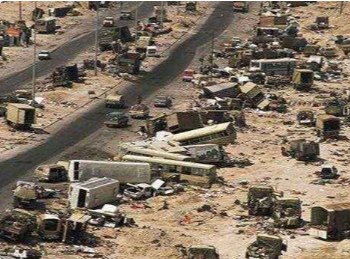
\includegraphics[scale=0.2]{figures/soft1}}\quad
				%\subfigure{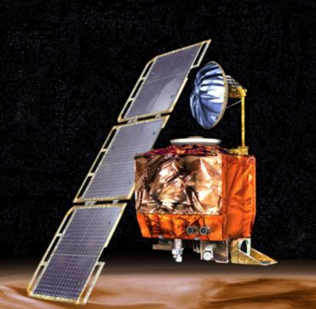
\includegraphics[scale=0.4]{figures/soft2}}
			  \subfigure{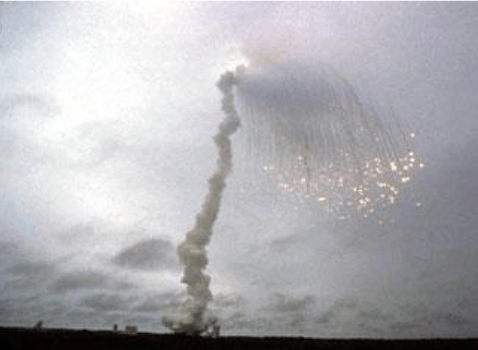
\includegraphics[scale=0.15]{figures/soft3}}\quad
				\subfigure{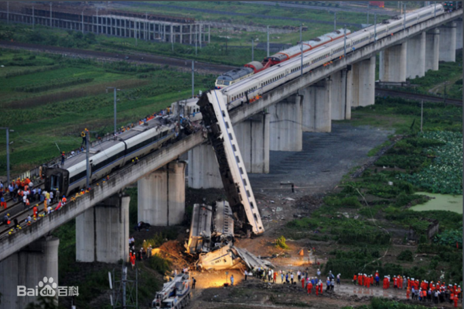
\includegraphics[scale=0.4]{figures/soft4}}
				\caption{系统故障引起的系列灾难现场}
			\end{figure}
			

			
			\only<1>{\begin{table}[htbp]
				\setlength{\abovecaptionskip}{-0.2cm}  %段前
				\setlength{\belowcaptionskip}{-0.4cm} %段后
				\fontsize{7pt}{\baselineskip}\selectfont
				\caption{由系统故障引起的重大事件概览}
				\label{tab:systemEvents_1.1}
				\centering
				\begin{tabular}{p{0.12\textwidth}p{0.35\textwidth}p{0.5\textwidth}}%
					\toprule
					\textbf{时间}&\textbf{事故原因}&\textbf{损失}\\
					\midrule
					1991年 & 美国爱国者导弹系统舍入错误 & 28名士兵死亡、100人受伤等\\
					1996年 & 阿丽亚娜5火箭 代码重用 & 火箭与其它卫星毁灭\\
					1999年 & 火星探测器用错度量单位 & 探测器坠毁并造成了3.27亿美元的损失\\
					2011年 & 温州7.23动车\underline{信号设备}在设计上存在严重的缺陷 &动车脱节脱轨、多人失去生命\\
					\bottomrule
				\end{tabular}
			\end{table}}
		\only<2>{\begin{block}
				系统正确对国防、太空勘测和交通运输至关重要。
		\end{block}}
	\end{frame}

	\begin{frame}
		\frametitle{研究背景和意义: {\small 形式化验证为系统的正确提供了有力依据}} 
\begin{block}{自动定理证明(Automated theorem proving)}
		\begin{columns}
		\column{0.5\textwidth}
			令$\phi_{imp}$和$\phi_{spec}$分别表示系统模型和规范对应的时序逻辑公式:
			\begin{itemize}
				\item $\phi_{imp} \rto \phi_{spec}$,或
				\item $\phi_{imp} \lrto \phi_{spec}$。
			\end{itemize}
		\column{0.5\textwidth}
			\begin{figure}
				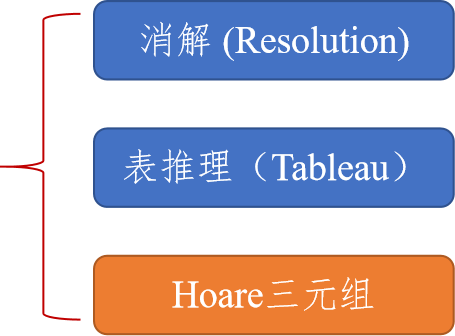
\includegraphics[scale=0.3]{figures/atp}
			\end{figure}
		\end{columns} 
	\begin{figure}
		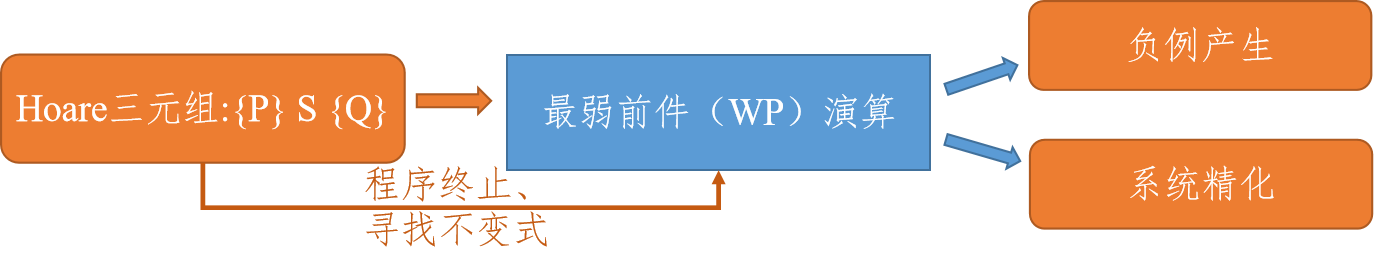
\includegraphics[scale=0.3]{figures/hoareTriple}
	\end{figure}
	\end{block}
\vskip 2pt
	\begin{block}{模型检测(Model Checking)}
		\begin{columns}
			\column{0.5\textwidth} 
			\begin{itemize}
				\item $\textcolor{red}{\Hm} \models^? \phi_{spec}$.
				\item {\small 反应式系统(reactive system):是指与环境有着持续不断交互的系统。}
				\item \textcolor{red}{如何计算反应式系统的WP?}
			\end{itemize}
			\column{0.5\textwidth}
			\begin{figure}
				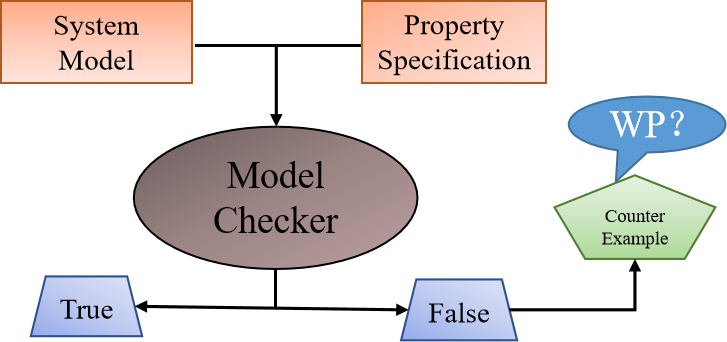
\includegraphics[scale=0.35]{figures/MC}
			\end{figure}
		\end{columns}
	\end{block}
	\end{frame}

\begin{frame}
	\frametitle{~研究背景和意义:{\small 简单的例子}}
	{\scriptsize \begin{example}[汽车制造企业模型]\label{car_manufacturing}
		
			一个汽车制造企业能够生产两种汽车:小轿车($se$)和跑车($sp$)。每隔一段时间,该企业都会做一个生产决策($d$),即:合理的生产计划。
			刚开始的时候,该企业做出了具有三个选择($s$)的方案:
			\begin{itemize}
				\item[(1)] 先生产足够的$se$,然后在再生产$sp$;
				\item[(2)] 先生产足够的$sp$,然后再生产$se$;
				\item[(3)] 同时生产$se$和$sp$。
			\end{itemize}
		这一过程可以由图~\ref{BVM}中的Kripke结构(带标签的状态转换图)$\Hm=(S,R,L)$形式化地展现出来,其中:
		\begin{columns}
			\column{0.5\textwidth}
			\begin{itemize}
				\item $V=\{d,s, se, sp\}$为该工厂所需要考虑的原子命题集;
				\item $S=\{s_0,s_1,s_2,s_3,s_4\}$为状态空间;
				\item $R = \{(s_0, s_1), (s_1,s_2), (s_1,s_3), (s_1,s_4),
				$ $(s_2,s_0),$ $(s_3,s_0),$ $(s_4,s_0)\}$ 为状态转换关系集;
				\item $L: S \rto 2^V$为标签函数,具体地:$L(s_0) = \{d\}$、$L(s_1) = \{s\}$、 $L(s_2)=\{se\}$、 $L(s_3) = \{sp\}$和$L(s_4) = \{se,sp\}$。
			\end{itemize}
			\column{0.5\textwidth}  
			 \begin{figure} 
			 	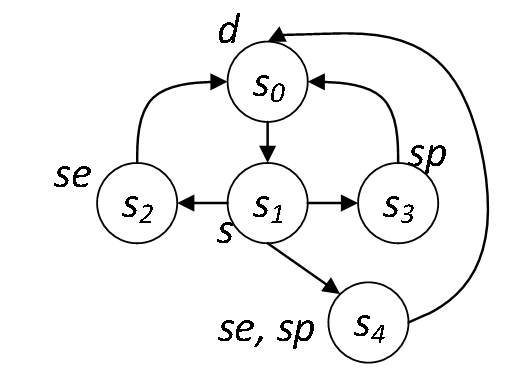
\includegraphics[width=3cm]{figures/NnewCar}
			 	\caption{汽车制造企业模型}\label{BVM}
			 \end{figure} 
		\end{columns} 
		假定,由于经济危机或者战略调整,导致该企业不能再生产跑车。这意味着所有规范和Kripke结构都不再需要考虑$sp$的,因此应该\textcolor{blue}{“移除”}。
	\end{example}}
\end{frame}
	
	\begin{frame}
		\frametitle{~研究背景和意义: {\small 知识表示与推理(KR)中的SNC和WSC}}
		{\small\begin{block}{最强必要条件(SNC)和最弱充分条件(WSC)}
			SNC和WSC分别用于描述给定理论下的最一般的结果(consequence)和最一般的诱因(abduction)[4]。满足下面两个条件的$\varphi$称为$q$在理论$\Sigma$下的SNC:
			\begin{itemize}
				\item[(1)] $\Sigma \models q \rto \varphi$;
				\item[(2)] 对任意$\varphi'$且$\Sigma \models q \rto \varphi'$,有$\Sigma \models \varphi \rto \varphi'$。
			\end{itemize}
		满足下面两个条件的$\psi$称为$q$在理论$\Sigma$下的(WSC):
		\begin{itemize}
			\item[(1)] $\Sigma \models \psi \rto q$; 
			\item[(2)] 对任意$\psi'$且$\Sigma \models \psi' \rto q$,有$\Sigma \models \psi' \rto \psi$。
		\end{itemize}
		\end{block}}
		\vskip 0.5pt
		{\small\begin{block}{遗忘理论(Forgetting)}
			\begin{columns}
				\column{0.5\textwidth} 
				 %在一阶逻辑中,从公式$\varphi$中遗忘掉一个$n$元谓词$P$的结果是$\exists R.\varphi[P/R]$,即将公式$\varphi$中的所有$P$的出现都用一个新的$n$元谓词$R$来替代。 
				 {\em 遗忘}是一种从理论中抽取知识的技术[5],被用于\underline{规划}[6,7]和\underline{知识更新}中[8]。非形式化地,对于逻辑语言L中的任意公式和原子集合,如果从该公式中遗忘掉该原子集合后得到的结果仍然在L中,则称\textcolor{blue}{遗忘存在},同时也称该公式和原子集合的遗忘存在。
				\column{0.5\textwidth}
				\begin{figure}
					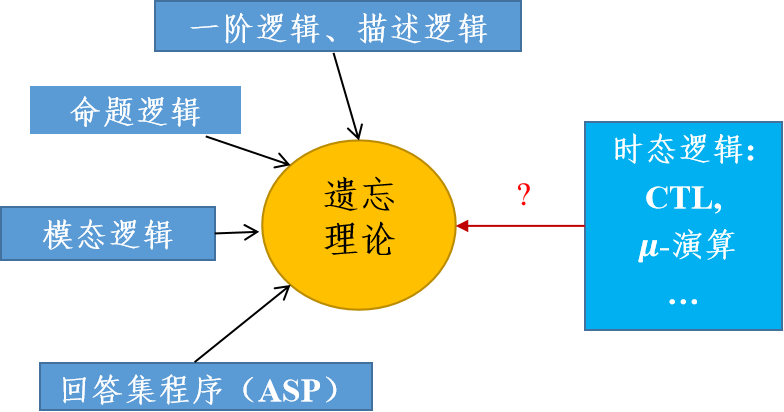
\includegraphics[scale=0.35]{figures/forgetting}
				\end{figure}
			\end{columns}
		\end{block}}
	\end{frame}
	
	\section{国内外研究现状} 
	%\subsection*{国内研究现状}
	\begin{frame}
		\frametitle{~国内外研究现状}
		\begin{figure}
			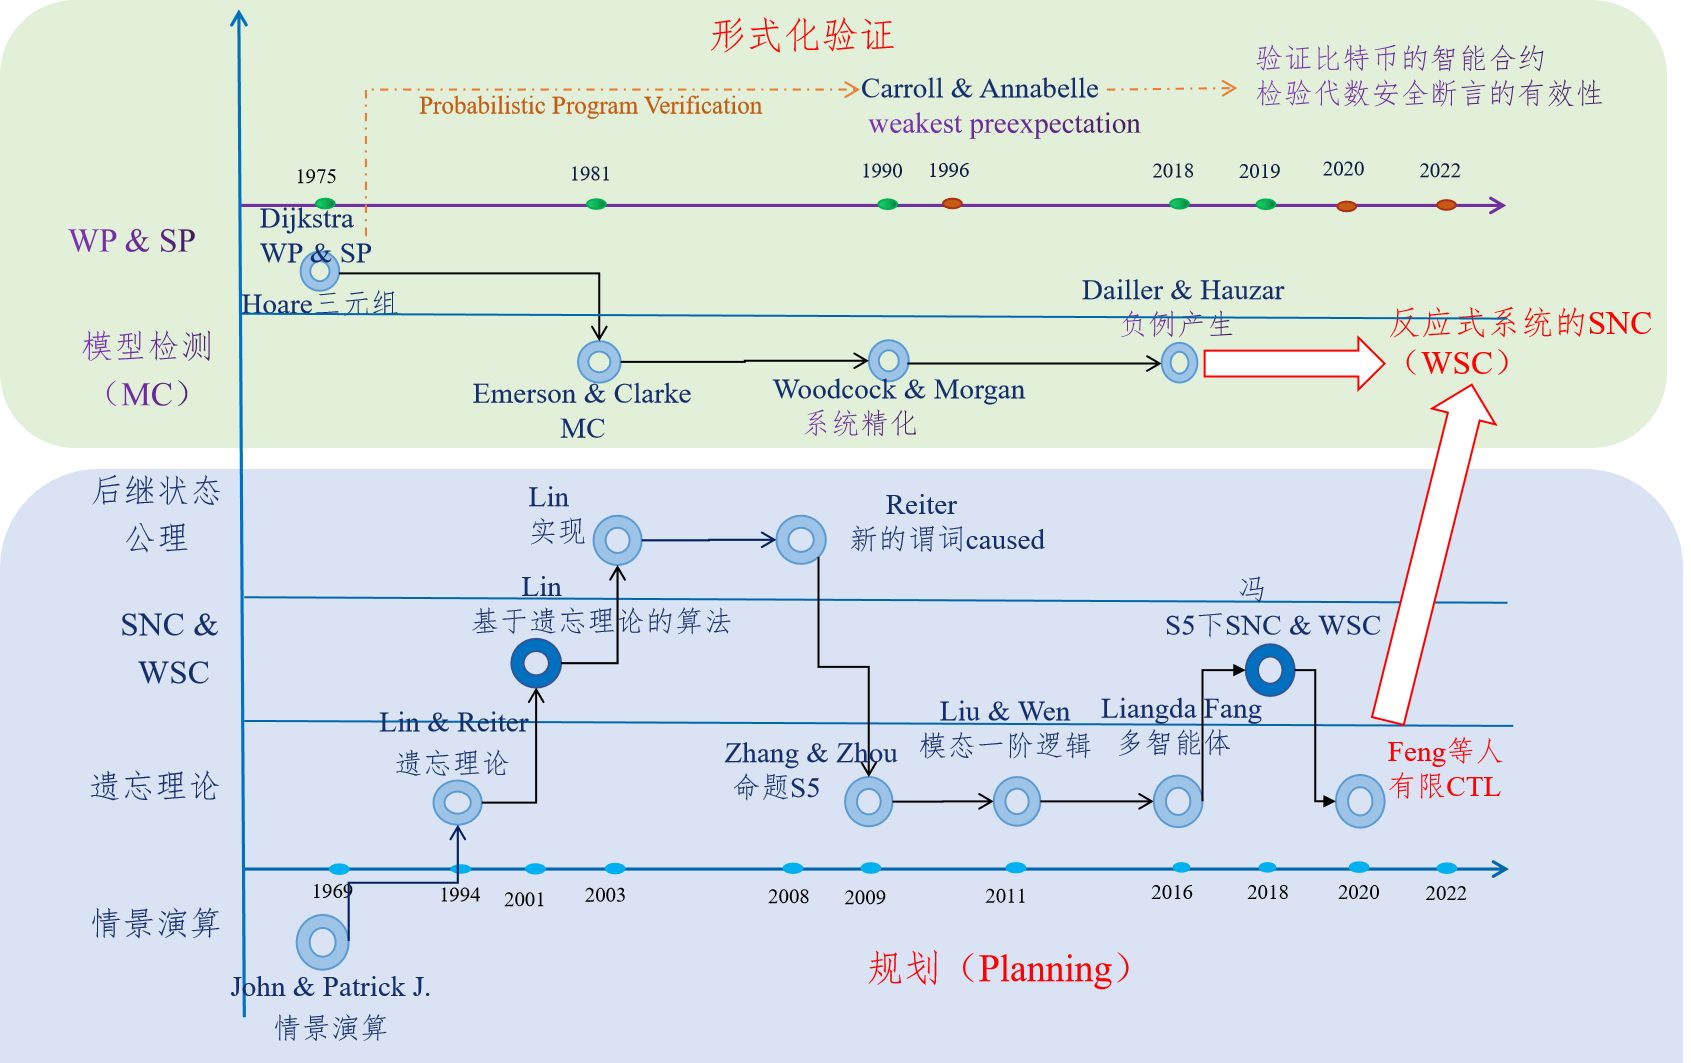
\includegraphics[scale=0.35]{figures/history1}
		\end{figure}
	\end{frame}
	
	\section{研究内容}
	\begin{frame}
		\frametitle{~研究内容}
		\begin{block}<1->{研究内容}
			\setlength{\baselineskip}{16pt}
			\uncover<1->{~~~本论文研究反应式系统下,$\CTL$和$\mu$-演算的遗忘理论,并使用遗忘计算WSC。具体为:}
			\begin{itemize}
				\vskip 8pt
				\item<2-> $\CTL$和$\mu$-演算的遗忘理论
				\begin{itemize}
					\item $\CTL$的遗忘理论
					\item $\mu$-演算的遗忘理论
				\end{itemize}
				\item<3-> 遗忘理论在反应式系统的形式化验证和知识更新中的应用
				\begin{itemize}
					\item 计算WSC和SNC
					\item 定义知识更新
				\end{itemize}
				\item<4-> 计算$\CTL$遗忘的算法
				\begin{itemize}
					\item 基于模型的计算方法
					\item 基于消解(resolution)的计算方法
					\item 实现与实验分析
				\end{itemize}
			\end{itemize}
		\end{block}
	\end{frame}

\begin{frame}
	\frametitle{~研究内容}
		\begin{itemize}
		\item  $\CTL$和$\mu$-演算的遗忘理论
		\item 遗忘理论在反应式系统的形式化验证和知识更新中的应用
		\item 计算$CTL$遗忘的计算方法
	\end{itemize}
	\begin{figure}
		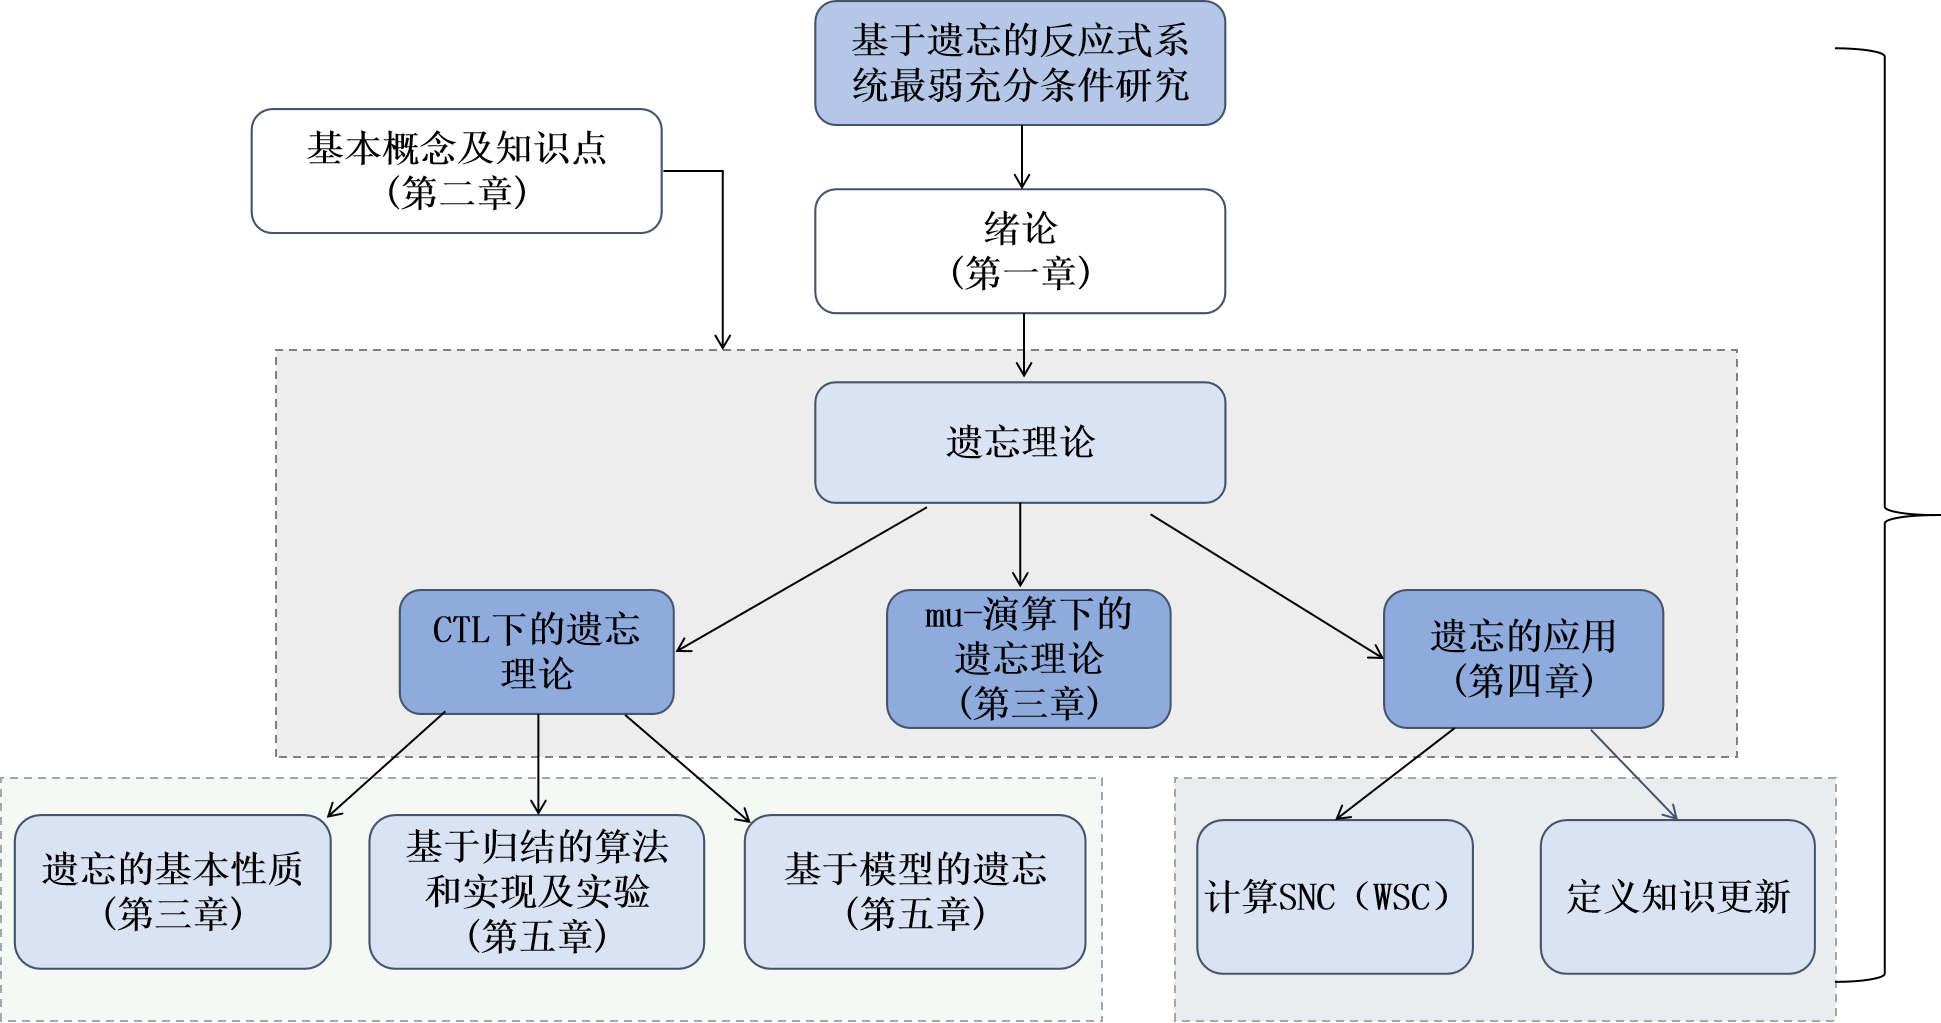
\includegraphics[scale=0.3]{figures/zuzhi1}
		\caption{文章组织结构示意图}
	\end{figure}
\end{frame}

\section{背景知识}
\subsection{Kripke结构}
\begin{frame}
	\frametitle{~Kripke结构}
{\footnotesize	
  $\Ha$:原子命题的集合 \qquad \qquad $\Ind$:索引的集合
	\begin{definition}[初始$\Ind$-Kripke结构]
		一个初始$\Ind$-Kripke结构是一个五元组$\Hm=(S,R,L,$ $[\_],s_0)$,其中:
		\begin{itemize}
			\item $S$是状态的非空集合,$s_0$是$\Hm$的初始状态(参见下文);
			\item $R \subseteq S \times S$是状态转换函数,且对任意$s\in S$,存在$s'\in S$使得$(s,s') \in R$;
			\item $L:S\rto 2^{\Ha}$是一个标签函数;
			\item $[\_]: \Ind \rto 2^{S \times S}$是一个函数,其使得对任意$ind \in\Ind$,若$s\in S$,则存在唯一一个$s\in S$使得$(s,s')\in [ind]\cap R$。
		\end{itemize}
	\end{definition}
	\only<1>{\begin{block}{相关概念}
		\begin{itemize}
			\item 初始Kripke结构$\Hm=(S,R,L,s_0)$:从初始$\Ind$-Kripke结构$\Hm$中去掉$[\_]$元素得到;
			\item $\Ind$-Kripke结构$\Hm=(S,R,L,[\_])$:从初始$\Ind$-Kripke结构$\Hm$中去掉初始状态$s_0$得到;
			\item Kripke结构$\Hm=(S,R,L)$:从初始$\Ind$-Kripke结构$\Hm$中同时去掉$[\_]$和$s_0$得到。
		\end{itemize}
	\end{block}}
	\only<2>{
		\begin{block}{相关概念}
			令$\Hm=(S,R,L)$为Kripke结构,$\Hm'=(S,R,L, [\_])$为$\Ind$-Kripke结构 :
			\begin{itemize}
				\item 路径:$\Hm$上的{\em 路径}是$\Hm$上的状态构成的无限序列$\pi=(s_0, s_{1}, s_{2},\dots)$,且满足对任意$j\ge 0$,$(s_j, s_{j+1}) \in R$;
				\item $s'\in \pi$:表示$s'$是路径$\pi$上的一个状态;  $\pi_{s}$:表示以$s$为起点的$\Hm$上的一条路径;
				\item 初始状态:如果对任意$s'\in S$,都存在路径$\pi_{s}$使得$s'\in \pi_{s}$,那么称$s$为\emph{初始状态};
				\item 索引路径:$\Hm'$上的一条\emph{索引路径}$\pi_{s}^{\tuple{ind}}$($ind \in \Ind$)是一条路径$(s_0(=s),$ $s_{1},$ $s_{2},$ $\dots)$,且对任意$j \geq 0$,有$(s_j, s_{j+1}) \in [ind]$。
			\end{itemize} 
		\end{block}
	}
	\only<3>{
		\begin{block}{相关概念}
		一个\emph{($\Ind$-)结构}是一个二元组${\cal K}=(\Hm, s)$,其中$\Hm$是一个初始($\Ind$-)Kripke结构,$s$是$\Hm$中的一个状态。
		如果$s$是$\Hm$的初始状态,则称${\cal K}$是{\em 初始 ($\Ind$-)结构}。
		
		在这些结构中,(索引)路径这一概念可以类似地定义。
		\end{block}
	}
}
\end{frame}


\subsection{CTL的语法和语义}
\begin{frame} 
	\frametitle{~$\CTL$的语法}
	{\footnotesize 
		\only<1>{\begin{block}{$\CTL$的语言符号}
			\begin{itemize}
				\item 原子命题集$\Ha$; \quad 可数无限索引集合$\Ind$;\quad 命题常量$\start$;
				\item 常量符号:$\top$和$\bot$,分别表示“真”和“假”;
				\item 联结符号:$\vee$和$\neg$,分别表示“析取”和“否定”;
				\item 路径量词:$\ALL$、$\EXIST$和$\EXIST_{ind}$,分别表示“所有”、“存在”和“存在索引为$ind\in \Ind$”的路径;
				\item 时序操作符:$\NEXT$、$\FUTURE$、$\GLOBAL$、$\UNTILL$和$\UNLESS$,分别表示“下一个状态”、“将来某一个状态”、“将来所有状态”、“直到”和“除非”;
				\item 标点符号:“(”和“)”。
			\end{itemize}
		\end{block}}
		\begin{definition}[带索引的$\CTL$]
			带索引的$\CTL$公式的\emph{存在范式(existential normal form, ENF)}可以用巴科斯范式递归定义如下:
			\begin{align*}
				\phi  ::= & \ \start\mid \bot %\mid \top
				\mid p \mid\neg\phi \mid \phi\lor\phi \mid
				\EXIST \NEXT \phi \mid
				\EXIST \GLOBAL \phi \mid 
				\EXIST (\phi\ \UNTILL\ \phi)\mid 
				\EXIST_{\tuple{ind}}\NEXT \phi  \mid 
				\EXIST_{\tuple{ind}}\GLOBAL \phi \mid
				\EXIST_{\tuple{ind}}(\phi \UNTILL \phi)  
			\end{align*}
		其中,$p\in \Ha$,$ind \in \Ind$。
		
		\textcolor{blue}{没有索引和$\start$的公式称为$\CTL$公式。}
		\end{definition}
	\only<2>{
		$\CTL$中其它形式的公式可以通过如下定义(使用上述定义中的形式)得到:
		\begin{alignat}{2}
			\varphi \wedge \psi& \ \overset{def}{=}\ \neg (\neg \varphi \vee \neg \psi)\\
			\varphi \rto \psi& \ \overset{def}{=}\ \neg \varphi \vee \psi\\
			\ALL(\varphi \UNTILL \psi)& \ \overset{def}{=}\ \neg\EXIST(\neg \psi \UNTILL(\neg \varphi \wedge \neg \psi)) \wedge \neg \EXIST \GLOBAL \neg \psi\\
			\ALL(\varphi \UNLESS \psi)& \ \overset{def}{=}\  \neg\EXIST((\varphi \wedge \neg \psi) \UNTILL (\neg \varphi \wedge \neg \psi))\\
			\EXIST(\varphi \UNLESS \psi)& \ \overset{def}{=}\  \neg\ALL((\varphi \wedge \neg \psi) \UNTILL (\neg \varphi \wedge \neg \psi))\\
			\ALL\FUTURE \varphi& \ \overset{def}{=}\ 	\ALL(\top \UNTILL \psi)\\
			\EXIST\FUTURE \varphi& \ \overset{def}{=}\ \EXIST(\top \UNTILL \psi)\\
			\ALL \NEXT \varphi& \ \overset{def}{=}\  \neg \EXIST \NEXT \neg \varphi\\
			\ALL \GLOBAL \varphi& \ \overset{def}{=}\  \neg \EXIST \FUTURE \neg \varphi
		\end{alignat}
	}
\only<3>{
	\begin{block}{符号优先级}
		带索引的$\CTL$中各类符号的优先级如下,且从左到右优先级逐渐降低:
		\begin{align*}
			& \neg, \EXIST\NEXT, \EXIST\FUTURE, \EXIST\GLOBAL, \ALL\NEXT, \ALL\FUTURE, \ALL\GLOBAL, \EXIST_{\tuple{ind}}\NEXT, \EXIST_{\tuple{ind}}\FUTURE, \EXIST_{\tuple{ind}}\GLOBAL
			,\land, \lor,
			\EXIST\UNTILL, \ALL\UNTILL, \EXIST \UNLESS, \ALL\UNLESS, \EXIST_{\tuple{ind}}\UNTILL, \EXIST_{\tuple{ind}} \UNLESS, \rto.
		\end{align*}
	
	此外,给定一个不包含“$\rto$”的公式$\varphi$和原子命题$p$。在$\varphi$中,若$p$的前面有偶数个否定$\neg$,则称$p$在$\varphi$中的出现为\emph{正出现},否则为\emph{负出现}。若$\varphi$中所有$p$的出现都为正出现(或负出现),则称$\varphi$关于$p$是正的(或负的)。
	\end{block}
}
	}
\end{frame}

\begin{frame} 
	\frametitle{~$\CTL$的语义}
	{\footnotesize 
		\only<1>{\begin{definition}[带索引的$\CTL$的语义]\label{def:ctl:semantic}
			给定公式$\varphi$,初始$\Ind$-Kripke结构 $\Hm=(S,R,L,[\_],s_0)$ 和状态 $s\in S$。$(\Hm,s)$与$\varphi$之间的可满足关系$(\Hm,s)\models \varphi$定义如下:
			\begin{itemize}
				\item $({\cal M},s) \models \start$ 当且仅当 $s=s_0$;
				\item $(\Hm,s) \not \models \bot$;%且$(\Hm, s) \models \top$;
				\item $(\Hm,s)\models p$ 当且仅当$p\in L(s)$;
				\item $(\Hm,s) \models \varphi_1 \vee \varphi_2$当且仅当$(\Hm,s)\models \varphi_1$或$(\Hm,s)\models \varphi_2$;
				\item $(\Hm,s)\models \neg \varphi$当且仅当$(\Hm,s)\not \models \varphi$;
				\item $(\Hm,s)\models \EXIST\NEXT \varphi$当且仅当存在$S$中的一个状态$s_1$,使得$(s,s_1)\in R$且$(\Hm,s_1)\models \varphi$;
				\item $(\Hm,s)\models \EXIST\GLOBAL\varphi$当且仅当存在$\Hm$上的一条路径$\pi_s=(s_1=s, s_2,\dots)$,使得对每一个$i\ge 1$都有$(\Hm,s_i)\models \varphi$;
				\item $(\Hm,s)\models \EXIST(\varphi \UNTILL \psi)$当且仅当存在$\Hm$上的一条路径$\pi_s=(s_1=s, s_2,\dots)$,使得对某一个$i\ge 1$有$(\Hm,s_i)\models \psi$,且对任意$1\leq j < i$,有$(\Hm,s_j)\models \varphi$;
				\item $({\cal M},s)\models \EXIST_{\tuple{ind}} \NEXT \psi$ 当且仅当对索引路劲$\pi_{s}^{\tuple{ind}}=(s,s',\dots)$, 有$(\Hm, s')\models \psi$;
				\item $({\cal M},s)\models \EXIST_{\tuple{ind}}\GLOBAL\psi$ 当且仅当
				对任意 $s' \in  \pi_{s}^{\tuple{ind}}$, %occurring in $\pi_{s}^{\tuple{ind}}$,
				$(\Hm,s') \models \psi$;
				\item $({\cal M},s)\models \EXIST_{\tuple{ind}}(\psi_1\UNTILL\psi_2)$ 当且仅当
				存在 $ \pi_{s}^{\tuple{ind}} = (s=s_1, s_2, \dots)$中的 $s_j$ ($1\leq j$)使得$(\Hm,s_j)$ $\models \psi_2$且对任意 $s_k \in \pi_{s}^{\tuple{ind}}$,若$1\leq k < j$,则 $(\Hm,s_k) \models \psi_1$。
			\end{itemize}
		\end{definition}}
	\only<2>{
	\begin{block}{记号}
		令$\varphi$、$\varphi_1$和$\varphi_2$为公式,这里列出文中出现的一些记号及其含义。
		\begin{itemize}
			\item $\Mod(\varphi)$:公式$\varphi$的所有模型构成的集合;
			\item 可满足:如果$\Mod(\varphi)\not = \emptyset$,则称$\varphi$是\emph{可满足}的;
			\item 逻辑蕴涵:若$\Mod(\varphi_1)\subseteq \Mod(\varphi_2)$,则称$\varphi_1$\emph{逻辑地蕴涵}$\varphi_2$,记为$\varphi_1\models \varphi_2$;
			\item 逻辑等值:当$\varphi_1\models \varphi_2$且$\varphi_2\models \varphi_1$时,即$\Mod(\varphi_1)= \Mod(\varphi_2)$,则称$\varphi_1$和$\varphi_2$为\emph{逻辑等值公式}(简称为\emph{等值公式}),记作$\varphi_1 \equiv \varphi_2$;
			\item $\Var(\varphi)$:出现在$\varphi$中的原子命题集;
			\item $\bigvee \Pi$和$\bigwedge \Pi$分别表示有限集$\Pi$中公式的析取和合取;
			\item \emph{$V$-无关}( \emph{$V$-irrelevant}):给定公式$\varphi$和原子命题集$V$,如果存在一个公式$\psi$使得$\Var(\psi) \cap V = \emptyset$且$\varphi \equiv \psi$,那么说$\varphi$与$V$中的原子命题\emph{无关},简称为\emph{$V$-无关}( \emph{$V$-irrelevant}),写作$\IR(\varphi,V)$。 
			\item 文字(literal)、子句(clause)、析取范式等跟经典命题情形中的定义一样。
		\end{itemize}
	\end{block}
}
	}
\end{frame}


\begin{frame} 
	\frametitle{~$\CTL$的标准形式法}
	{\footnotesize 
		\only<1>{\begin{block}{$\CTLsnf$子句}
			具有下面几种形式的公式称为$\CTL$全局子句分离范式(separated normal form with global clauses for \CTL,$\CTLsnf$子句)\cite{zhang2008first,zhang2014resolution}:
			\[
			\begin{array}{ll}
				\ALL \GLOBAL (\start \rto \bigvee_{j=1}^{k} m_{j}) & \text{(初始句,initial clause)} \\
				\ALL \GLOBAL (\top\rto \bigvee_{j=1}^{k} m_{j}) &\text{(全局子句,global clause)} \\
				\ALL \GLOBAL (\bigwedge_{i=1}^{n} l_{i} \rto \ALL \NEXT \bigvee_{j=1}^{k} m_{j}) & (\ALL\text{-步子句,} \ALL\text{-step clause}) \\
				\ALL \GLOBAL (\bigwedge_{i=1}^{n} l_{i} \rto \EXIST_\tuple{ind} \NEXT \bigvee_{j=1}^{k} m_{j}) & (\EXIST\text{-步子句,} \EXIST\text{-step clause}) \\
				\ALL \GLOBAL (\bigwedge_{i=1}^{n} l_{i} \rto \ALL \FUTURE l) & (\ALL\text{-某时子句,} \ALL\text{-sometime clause}) \\
				\ALL \GLOBAL (\bigwedge_{i=1}^{n} l_{i} \rto \EXIST_{\tuple{ind}} \FUTURE l) & (\EXIST\text{-某时子句,} \EXIST\text{-sometime clause})\\
			\end{array}
			\]
			其中$k$和$n$都是大于0的常量,$l_i$($1\leq i \leq n$)、$m_j$($1\leq j \leq k$)和$l$都是文字且$ind \in \Ind$。
		\end{block}}
	\only<2>{
		\begin{block}{转换规则}
			一个$\CTL$公式$\varphi$可以通过下表中的规则转换为一个$\CTLsnf$子句集,记为$T_{\varphi}$。
			
			\begin{table}%[width=.9\linewidth,cols=4,pos=h]
				\tiny
				\centering\caption{转换规则}\label{tab:trans}
				\begin{tabular}{c}
					\toprule
					$
					\begin{aligned}
						& \textbf{Trans(1)}\frac{q \rto \EXIST T \varphi}{q\rto \EXIST_{\tuple{ind}} T \varphi}; \qquad
						\textbf{Trans(2)} \frac{q \rto \EXIST (\varphi_1 \UNTILL \varphi_2)}{q\rto \EXIST_{\tuple{ind}} (\varphi_1 \UNTILL \varphi_2)};
						&& 
						\textbf{Trans(3)} \frac{q\rto \varphi_1 \wedge \varphi_2}{q\rto \varphi_1, q\rto \varphi_2};\\
						&   \textbf{Trans(4)}  \frac{q\rto \varphi_1 \vee \varphi_2\ (\hbox{如果$\varphi_2$不是子句})}{ q\rto \varphi_1 \vee p, p\rto \varphi_2};
						&&\textbf{Trans(5)}  \frac{q\rto D}{\top \rto \neg q \vee D};\ \frac{q\rto \perp}{ \top \rto \neg q};\ \frac{q \rto \top}{\{\}} \\
						&  \textbf{Trans(6)} \frac{q\rto Q\NEXT \varphi\ (\hbox{如果$\varphi$不是子句})}{q\rto Q\NEXT p, p\rto \varphi}; 
						&& \textbf{Trans(7)} \frac{q\rto Q\FUTURE \varphi\ (\hbox{如果$\varphi$不是文字})}{q\rto Q\FUTURE p, p\rto \varphi}; \\
						&  \textbf{Trans(8)} \frac{q\rto Q(\varphi_1 \UNTILL \varphi_2) \  (\hbox{如果$\varphi_2$不是文字})}{q\rto Q(\varphi_1 \UNTILL p),  p\rto \varphi_2}; 
						&& \textbf{Trans(10)} \frac{q\rto Q\GLOBAL \varphi}{\ q \rto  p, p\rto \varphi,p\rto Q\NEXT p};\\
						& \textbf{Trans(9)} \frac{q\rto Q(\varphi_1 \UNLESS \varphi_2)\ (\hbox{如果 $\varphi_2$ 不是文字})}{q\rto Q(\varphi_1 \UNLESS p), p\rto \varphi_2}; &&\\  
						& \textbf{Trans(11)} \frac{q\rto Q(\varphi \UNTILL l)}{q \rto l\vee p, p\rto \varphi, p\rto Q\NEXT(l\vee p),q\rto Q \FUTURE l};
						&& \textbf{Trans(12)} \frac{q\rto Q(\varphi \UNLESS l)}{q \rto l\vee p, p\rto \varphi, p\rto Q\NEXT(l\vee p)}.
					\end{aligned}
					$\\
					\bottomrule
				\end{tabular}
			\end{table}
			其中,$T\in \{\NEXT, \GLOBAL, \FUTURE\}$,$ind$是规则中引入的新索引且$Q\in \{\ALL, \EXIST_{\tuple{ind}}\}$;
			$q$是一个原子命题, $l$是一个文字, $D$是文字的析取(即子句), $p$是新的原子命题;$\varphi$,$\varphi_1$,和$\varphi_2$都是$\CTL$公式。
		\end{block}
	}
	\only<3>{
		\begin{block}{转换步骤}
			给定一个$\CTL$公式$\varphi$,将其转换为一个$\CTLsnf$字句集合的主要步骤如下:
			\begin{itemize}
				\item[(1)]  将公式$\CTL$转换为其NNF~\footnote{对于给定的公式$\varphi$,其否定范式(negation normal form, NNF)是将否定联结词“$\neg$”的出现通过上述定义变化到只出现在原子命题之前的形式。} 
				形式,记为$nnf(\varphi)$;
				\item[(2)]  使用等值公式化简$nnf(\varphi)$,得到$simp(nnf(\varphi))$;
				\item[(3)] 使用转换规则将$\{\ALL\GLOBAL(\start\rto z), \ALL\GLOBAL(z \rto simp(nnf(\varphi)))\}$化简为$\CTLsnf$子句集$T_{\varphi}$, 
				其中$T_\varphi$由如下\emph{导出(derivation)}序列生成:
				\[ T_0=\{\ALL\GLOBAL(\start\rto p), \ALL\GLOBAL(p\rto {\bf simp}({\bf nnf}(\varphi)))\}, T_1, \ldots, T_n=T_\varphi\]
				使得
				\begin{itemize}
					\item $p$是一个新的原子命题, 即:$p\notin \{\start\}\cup\Var(\varphi)$;
					\item $T_{t+1} = (T_t - \{\psi\}) \cup R_t~(t\ge 0)$,其中 $\psi$为$T_t$中的非$\CTLsnf$子句,且 $R_t$
					是使用一条匹配的归则作用到 $\psi$上得到的结果集;
					\item  $T_n$中的每个公式都是$\CTLsnf$子句形式。
				\end{itemize}
			\end{itemize}
		\end{block}
	}
	}
\end{frame}

\begin{frame}
	\frametitle{~例子}
	\begin{example}\label{exmp:transbot}
		\tiny
		令$\varphi=\neg \ALL \FUTURE p \wedge \ALL\FUTURE(p \wedge \top)$,下面给出将$\varphi$转换为$\CTLsnf$子句集的详细步骤。
		
		(1) 将公式$\varphi$转换为其NNF形式:$\EXIST\GLOBAL \neg p \wedge \ALL\FUTURE(p \wedge \top)$;
		
		(2) 化简(1)中的公式为:$\EXIST\GLOBAL \neg p \wedge \ALL\FUTURE p$;
		
		(3) 使用转换规则转换$\{\ALL\GLOBAL(\start \rto z), \ALL\GLOBAL(z \rto (\EXIST\GLOBAL \neg p \wedge \ALL\FUTURE p))\}$,详细步骤如下:
		\begin{align*}
			&1.\ \start \rto z && \\
			&2.\ z \rto \EXIST\GLOBAL \neg p \wedge \ALL\FUTURE p &&  \\
			% \end{align*}
			% \begin{align*}
			&3.\ z \rto  \EXIST\GLOBAL \neg p && (2, \textbf{Trans(3)})\\
			&4.\ z \rto \ALL\FUTURE p && (2, \textbf{Trans(3)})\\
			&5.\ z \rto  \EXIST_{\tuple{1}}\GLOBAL \neg p  && (3, \textbf{Trans(1)})\\
			&6.\ z \rto x && (5, \textbf{Trans(10)})\\
			&7.\ x\rto \neg l && (5, \textbf{Trans(10)})\\
			&8.\ x\rto \EXIST_{\tuple{1}} \GLOBAL x&& (5, \textbf{Trans(10)})\\
			&9.\ \top \rto \neg z \vee x && (6, \textbf{Trans(5)}) \\
			% \end{align*}
			% \begin{align*}
			&10.\ \top \rto \neg x \vee \neg p && (7, \textbf{Trans(5)}) 
		\end{align*}
		
		因此,得到的$\varphi$对应的$\CTLsnf$子句集为:
		\begin{align*}
			&1.\ \start \rto z && 2.\ z \rto \ALL\FUTURE p && 3.\ x\rto \EXIST_{\tuple{1}} \GLOBAL x
			&& 4.\ \top \rto \neg z \vee x && 5.\ \top \rto \neg x \vee \neg p.
		\end{align*}
	\end{example}
\end{frame}

\subsection{$\mu$-演算}
\begin{frame} 
	\frametitle{~$\mu$-演算的语法}
	{\footnotesize 
		不动点符号:$\mu$和$\nu$,分别表示“最小不动点”和“最大不动点”。
		
		${\cal V}$:变元符号的可数集。
		
		各类符号之间的优先级如下(从左到右优先级逐渐变低):
		\[
		\neg\qquad \EXIST\NEXT\qquad \ALL\NEXT\qquad \wedge\qquad \vee\qquad \mu \qquad \nu.
		\]
	\begin{definition}[$\mu$-演算公式]
		$\mu$-演算公式(简称为$\mu$-公式或公式)递归定义如下:
		\[
		\varphi ::=   p\mid  X\mid \neg \varphi\mid \varphi \vee \varphi \mid \ALL\NEXT \varphi\mid  \nu X. \varphi
		\]
		其中$p\in \Ha$且$X\in {\cal V}$。
	\end{definition}
\only<1>{
	\begin{block}{约定}
		\begin{itemize}
			\item 公式$\nu X.\varphi$中的$X$总是正出现在$\varphi$中,即:$\varphi$中$X$的每一次出现之前都有偶数个否定符号“$\neg$”;
			\item 称出现在$\mu X. \varphi$和$\nu X. \varphi$中的变元$X$是\emph{受约束的}(bound),且受约束的变元称为{\em 约束变元},不受约束的变元称为\emph{自由变元};
			\item 文字(literal):原子命题和变元符号及其各自的否定;
			\item 这里所谈到的公式指的是取名恰当的(well-named)、受保护(guarded)的$\mu$-公式。
		\end{itemize}
	\end{block}
}
\only<2>{
	\begin{block}{注意}
		在$\mu$-演算公式的定义中,通常考虑动作集$Act$和一组与$a\in Act$相关的模态词“$\tuple{a}$”\cite{DBLP:journals/cacm/Kozen83,d1996uniform,d2000logical}。为了方便,本文考虑公式里只有一个动作的情形,但是本文的结论可以扩展到一般的情形。此时,模态词中的动作$a$可以省略,且公式$\EXIST\NEXT\varphi$(或$\ALL\NEXT \varphi$)与公式 $\tuple{a}\varphi$(或$[a]\varphi$)\cite{d2000logical}相同。
	\end{block}
}
}
\end{frame}
\begin{frame}
	\frametitle{$\mu$-演算的语义}
	{\footnotesize 
	\begin{definition}
		给定$\mu$-演算公式$\varphi$、Kripke结构$\Hm=(S,R,L,r)$和一个从${\cal V}$中的变量到$\Hm$中状态的赋值函数$v: {\cal V} \rto 2^S$。公式在$\Hm$和$v$上的解释是$S$的一个子集$\left\| \varphi\right\|_v^{\Hm}$(如果在上下文中$\Hm$是明确的,则可以省去上标):
		\begin{align*}
			& \left \| p\right \|_v = \{s\mid p \in L(s)\}, \\  
			& \left\| X\right\|_v = v(X),\\
			& \left\|\varphi_1 \vee \varphi_2\right\|_v = \left\|\varphi_1\right\|_v \cup \left\|\varphi_2\right\|_v,\\ 
			& \left\|\ALL \NEXT \varphi\right\|_v = \{s\mid \forall s'. (s, s') \in R \Rto s' \in \left\|\varphi\right\|_v\},\\ 
			& \left\| \nu X. \varphi\right\|_v = \bigcup\{S' \subseteq S \mid S' \subseteq \left\|\varphi\right\|_{v[X:= S']}\}.
		\end{align*}
		其中,$v[X:= S']$是一个赋值函数,它除了$v[X:= S'](X)=S'$之外,和$v$完全相同。
	\end{definition}
\only<1>{\textbf{注意:}虽然这里的Kripke结构不要求其二元关系是完全的,但是这里的情况更加一般化,其结论也能推广到二元关系是完全的情形。}
\only<2>{
	\begin{block}{记号和约定}
		\begin{itemize}
			\item 赋值:由$\Hm$、其赋值函数$v$和$\Hm$上的状态$s$构成的三元组$(\Hm,s,v)$称为为{\em 赋值}(当$s$为$\Hm$的根时,$(\Hm,s,v)$简写为$(\Hm,v)$,也称其为一个赋值);
			\item 若$s\in \left\| \varphi \right\|_v$,则称$s$“满足”$\varphi$,记为$(\Hm, s, v) \models \varphi$;
			\item $\Mod(\varphi)$:$\varphi$的模型的集合,即$\Mod(\varphi) = \{(\Hm,v) \mid (\Hm,r,v) \models \varphi\}$(当$\varphi$为$\mu$-句子时,也可简写为$\Mod(\varphi) = \{\Hm\mid (\Hm,r,v) \models \varphi\}$);
			\item 当公式$\varphi$为$\mu$-句子时,可以将赋值函数$v$省略。
		\end{itemize}
	\end{block}
}
}
\end{frame}

\begin{frame}
	\frametitle{$\mu$-公式的析取范式}
	{\footnotesize
		\begin{block}{$\mu$-演算的覆盖-语法}
			在覆盖-语法语法中,用\emph{覆盖操作}(cover operator)集替换上述$\mu$-公式的定义中的$\EXIST\NEXT$,且满足
			\begin{itemize}
				\item $Cover(\emptyset)$是公式;
				\item 对任意$n\geq 1$,若$\varphi_1,\dots, \varphi_n$是公式,则$Cover(\varphi_1, \dots, \varphi_n)$是公式。
			\end{itemize}
		\end{block}
		\only<1>{\begin{definition}
			对于给定的初始结构$\Hm=(S,R,L,r)$和赋值函数$v$:
			\begin{itemize}
				\item $(\Hm,r,v) \models Cover(\emptyset)$当且仅当$r$没有任何的后继状态;
				\item $(\Hm, s,v ) \models Cover(\varphi_1, \dots, \varphi_n)$当且仅当
				\begin{itemize}
					\item 对任意$i = 1, . . . , n$,存在$(s, t) \in R$使得$(\Hm, t,v) \models \varphi_i$;
					\item 对任意$(s, t) \in R$,存在$i\in \{1, . . . , n\}$使得$(\Hm, t,v) \models \varphi_i$。
				\end{itemize}
			\end{itemize}
		\end{definition}}
	\only<2>{
		\begin{block}{等价关系}
			覆盖-语法与上述$\mu$-演算的语法是等价的\cite{d2006modal},且$Cover$公式与$\EXIST\NEXT$公式之间可以通过下面的等式转换:
			\[
			Cover(\varphi_1, \dots, \varphi_n) \LRto \EXIST\NEXT \varphi_1 \wedge \dots \wedge \EXIST\NEXT \varphi_n \wedge \ALL\NEXT(\varphi \vee \dots \vee \varphi_n),
			\]
			反之,
			\[
			\EXIST\NEXT \varphi \LRto Cover(\varphi, \top).
			\]
		\end{block}
	}
	\only<3>{
		\begin{definition}[析取$\mu$-公式~\cite{d2006modal}]
			析取$\mu$-公式集${\cal F}_d$是包含$\top$、$\bot$和不矛盾的文字的合取且封闭于下面几条规则的最小集合:
			\begin{itemize}
				\item[(1)] 析取式(disjunctions):若$\alpha, \beta \in {\cal F}_d$,则$\alpha \vee \beta \in {\cal F}_d$;
				\item[(2)] 特殊合取式(special conjunctions):若$\varphi_1, \dots, \varphi_n\in {\cal F}_d$且$\delta$为不矛盾的文字的合取,则$\delta \wedge Cover(\varphi_1, \dots, \varphi_n) \in {\cal F}_d$;
				\item[(3)] 不动点操作(fixpoint operators):若$\varphi\in  {\cal F}_d$,且对任意公式$\psi$,$\varphi$不含有形如$X \wedge \psi$的子公式,则$\mu X. \varphi$和$\nu X. \varphi$都在 ${\cal F}_d$中。
			\end{itemize}	
		\end{definition}
	}
	}
\end{frame}
	
	\section{CTL和mu-演算遗忘理论}
	\subsection*{CTL遗忘理论}
	\begin{frame}
		\frametitle{~CTL遗忘理论}
		{\scriptsize 
			\begin{definition}[$V$-互模拟]
				\label{def:VInd:bisimulation}
				给定原子命题集$V\subseteq\cal A$、索引集合$I\subseteq \Ind$和初始$\Ind$-结构 $\Hm_i=(S_i, R_i,L_i, [\_]_i, s_0^i)~(i=1,2)$。
				$\Hb_V \subseteq S_1 \times S_2$为二元关系,对任意$s_1 \in S_1$和$s_2 \in S_2$,若$(s_1, s_2)\in \Hb_V$,则:
				\begin{itemize}
					\item[(i)] $L_1(s_1) - V = L_2(s_2) -V$;
					\item[(ii)] $\forall r_1\in S_1$, 若$(s_1, r_1)\in R_1$,则$\exists r_2 \in S_2$ 使得 $(s_2,r_2) \in R_2$ 和 $(r_1, r_2) \in \Hb_V$;
					\item[(iii)] $\forall r_2\in S_2$,若$(s_2, r_2)\in R_2$,则 $\exists r_1 \in S_1$ 使得 $(s_1,r_1) \in R_1$ 和 $(r_1, r_2)\in \Hb_V$。
				\end{itemize}
				那么,称 $\Hb_V$ 是 $\Hm_1$和 $\Hm_2$之间的一个 $V$-互模拟关系。
			\end{definition}
		\only<1>{\begin{columns}
			\column{0.5\textwidth} 
			\begin{itemize}
				\item 结构互模拟:若$\Hm_1$和 $\Hm_2$之间存在一个 $V$-互模拟关系$\Hb_V$使得$(s_1, s_2)\in \Hb_V$,则称两个 $\Ind$-结构 ${\cal K}_1$ $= (\Hm_1, s_1)$ 和 ${\cal K}_2 = (\Hm_2, s_2)$ 是 $V$-{\em 互模拟}的,记为${\cal K}_1$ $\lrto_V {\cal K}_2$;
				\item 路径互模拟:令$i\in \{1,2\}$,$\pi_i=(s_{i,1},$ $s_{i,2},\ldots)$ 为 $\Hm_i$ 上的路径,若对任意$j \ge 1$都有$ {\cal K}_{1,j} \lrto_V {\cal K}_{2,j}$,则称这两条路径是$V$-{\em 互模拟}的,记为$\pi_1 \lrto_V \pi_2$,其中 ${\cal K}_{i,j}=(\Hm_i,$ $s_{i,j})$。
			\end{itemize}
			\column{0.5\textwidth}
			\begin{figure}
				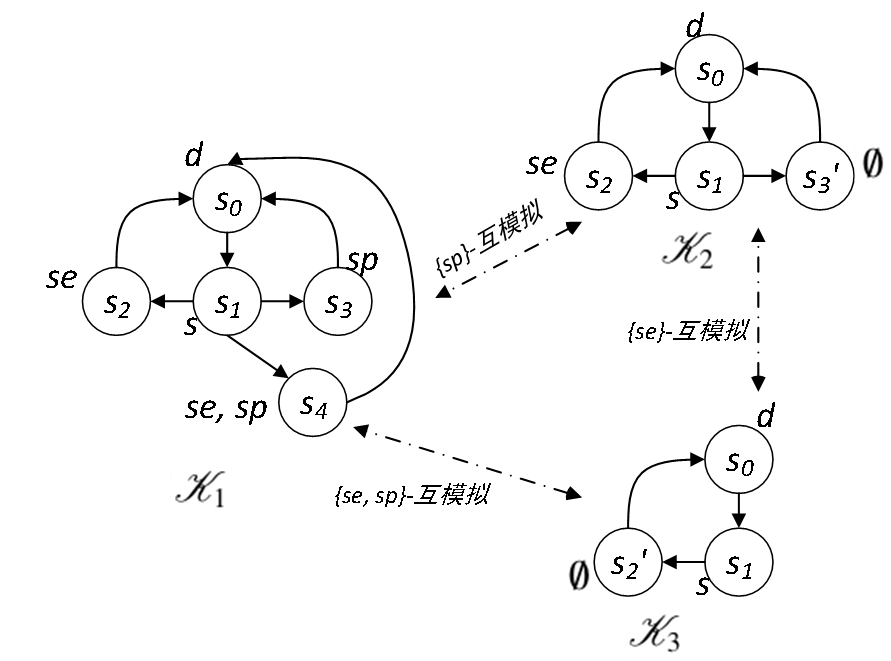
\includegraphics[scale=0.34]{figures/NVBnewCar1}
			\end{figure}
		\end{columns}}
	\only<2>{
	%	\begin{block}{相关性质 1} 
			\begin{proposition}
				给定集合$V_i\subseteq \Ha$、状态$s_i'$、路径$\pi_i'$和$\Ind$-结构${\cal K}_j=(\Hm_j,s_j)$,其中$i=1,2$,$j=1,2,3$。 
				如果${\cal K}_1 \lrto_{V_1} {\cal K}_2$且${\cal K}_2 \lrto_{V_2} {\cal K}_3$,则:
				\begin{itemize}
					\item[(i)] ${\cal K}_1\lrto_{V_1\cup V_2}{\cal K}_3$;
					\item[(ii)] 若 $V_1 \subseteq V_2$,则 ${\cal K}_1 \lrto_{V_2} {\cal K}_2$;
					\item[(iii)] $s_1'\lrto_{V_i}s_2'~(i=1,2)$ 蕴涵$s_1'\lrto_{V_1\cup V_2}s_2'$;
					\item[(iv)] $\pi_1'\lrto_{V_i}\pi_2'~(i=1,2)$ 蕴涵 $\pi_1'\lrto_{V_1\cup V_2}\pi_2'$;
					\item[(v)] 对$\Hm_1$上的每条路径 $\pi_{s_1}$,存在$\Hm_2$上的一条路径 $\pi_{s_2}$ 使得 $\pi_{s_1} \lrto_{V_1} \pi_{s_2}$,反之也成立。
				\end{itemize}
			\end{proposition}
	%	\end{block}
	}
	\only<3>{
		\begin{theorem}\label{thm:V-bisimulation:EQ}
			令$V\subseteq \Ha$是原子命题集,${\cal K}_i$ $(i=1,2)$是两个具有$V$-互模拟关系的$\Ind$-结构,即:${\cal K}_1 \lrto_V {\cal K}_2$。若$\Phi$是一个$\CTL$公式且$\IR(\Phi, V)$,则有${\cal K}_1\models \Phi$当且仅当${\cal K}_2\models \Phi$。
		\end{theorem}
	}
		}
	\end{frame}

\begin{frame}
	\frametitle{~互模拟等价}
	{\footnotesize
		\begin{definition}[互模拟等价,bisimilar equivalence]\label{def:bisimular:equivalene}
			给定原子命题集$V\subseteq {\cal A}$,公式$\varphi$和$\psi$。若对任意${\cal K}\models \varphi$,都存在一个${\cal K}'\models\psi$,使得${\cal K}\lrto_V{\cal K}'$;且对任意${\cal K}'\models\psi$,都存在一个${\cal K}\models \varphi$,使得${\cal K}\lrto_V{\cal K}'$,则称公式$\varphi$和 $\psi$是 {\em $V$-互模拟等价的(bisimilar equivalence)},记为 $\varphi\equiv_V\psi$。
		\end{definition}
	\only<1>{\begin{lemma}~\label{lem:eqR}
		对任意$V\subseteq\cal A$,  $\lrto_V$和 $\equiv_V$为等价关系。
	\end{lemma}}
\only<2>{
	\begin{corollary}~\label{cor:eqbi}
		令 $V$、$V_1$、$V_2$ 为$\cal A$的子集,$\varphi$和 $\psi$为公式。
		\begin{itemize}
			\item[(i)] 若 $\varphi\equiv\psi$,则 $\varphi\equiv_V\psi$。
			\item[(ii)] 若$\varphi$ 和 $\psi$不包括索引,且 $\varphi\equiv_\emptyset\psi$, 则 $\varphi\equiv\psi$。
			\item[(iii)] 若 $\varphi\equiv_{V_i}\psi~(i=1,2)$,则 $\varphi\equiv_{V_1\cup V_2}\psi$。
			\item[(iv)] 若 $\varphi\equiv_{V_1}\psi$ 和 $V_1\subseteq V_2$,则 $\varphi\equiv_{V_2}\psi$。
		\end{itemize}
	\end{corollary}
}
\only<3>{
	\begin{proposition}\label{prop:transform:V:EQ}
		令 $\varphi$为一个$\CTL$公式。则$\varphi\equiv_UT_\varphi$,其中 $T_\varphi=\CTLsnf(\varphi)$和
		$U=\Var(T_\varphi)-\Var(\varphi)$。
	\end{proposition}
}
	}
\end{frame}
	
	\begin{frame}{手牌拆分算法模块}
		\text{{\textbf{基于“斗地主”规则的拆分Split算法}}}
		\begin{figure}
			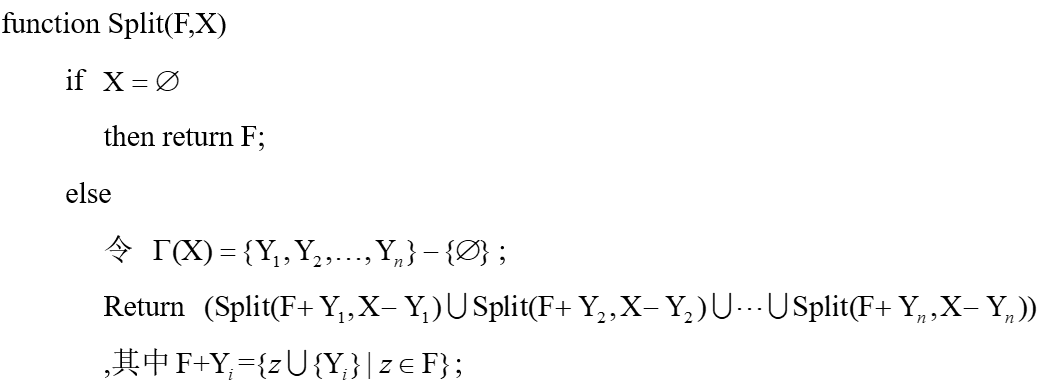
\includegraphics[scale=0.28]{figures/split}
		\end{figure}
	\end{frame}
	
	\begin{frame}{手牌拆分算法模块}
		\text{{\textbf{基于“斗地主”规则的手牌较小拆分算法(LessSplit)}}}
		\begin{figure}
			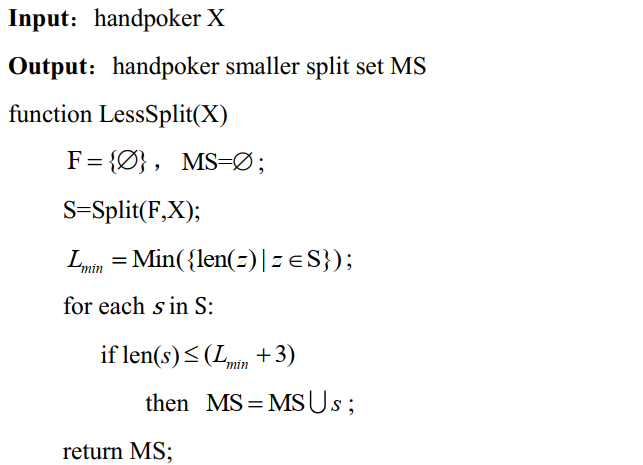
\includegraphics[scale=0.4]{figures/jiyushoupai}
		\end{figure}
	\end{frame}
	
	\begin{frame}
		\frametitle{~~手牌拆分算法实例}
		\begin{itemize}
			\item 玩家的手牌为: 34556789LB。对玩家手牌进行拆分,所有拆分结果为:
			\begin{itemize}
				\item<2-> $s_1$=\{3,4, 5, 5, 6,7, 8, 9, L, B\}
				\item<2-> $s_2$=\{3, 4, 5, 5, 6, 7, 8, 9, LB\}
				\item<2-> $s_3$=\{3, 4, 55, 6, 7, 8, 9, L, B\}
				\item<2-> $s_4$=\{3, 4, 55, 6, 7, 8, 9, LB\}
				\item<2-> $s_5$=\{3, 4, 5, LB, 56789\}
				\item<2-> $s_6$=\{3, 4, 5, L, B, 56789\}
				\item<2-> $s_7$=\{3, 5, 9, LB, 45678\}
				\item<2-> $s_8$=\{3, 5, 9, L, B, 45678\}
				\item<2-> $s_9$=\{3, 5, LB, 456789\}
				\item<2-> $s_{10}$=\{3, 5, L, B, 456789\}
				\item<2-> $s_{11}$=\{5, 8, 9, LB, 34567\}
				\item<2-> $s_{12}$=\{5, 8, 9, L, B, 34567\}
				\item<2-> $s_{13}$=\{5, 9, LB, 345678\}
				\item<2-> $s_{14}$=\{5, 9, L, B, 345678\}
				\item<2-> $s_{15}$=\{5, LB, 3456789\}
				\item<2-> $s_{16}$=\{5, L, B, 3456789\}
			\end{itemize}
		\end{itemize}
	\end{frame}
	
	
	\begin{frame}
		\frametitle{~~手牌拆分算法实例}
		\begin{itemize}
			\item 玩家的手牌为: 34556789LB。对玩家手牌进行拆分,所有拆分结果为:
			\begin{itemize}
				\item<1-> $s_1$=\{3,4, 5, 5, 6,7, 8, 9, L, B\}
				\item<1-> $s_2$=\{3, 4, 5, 5, 6, 7, 8, 9, LB\}
				\item<1-> $s_3$=\{3, 4, 55, 6, 7, 8, 9, L, B\}
				\item<1-> $s_4$=\{3, 4, 55, 6, 7, 8, 9, LB\}
				\item<1-> $s_5$=\{3, 4, 5, LB, 56789\}
				\item<1-> $s_6$=\{3, 4, 5, L, B, 56789\}
				\item<1-> $s_7$=\{3, 5, 9, LB, 45678\}
				\item<1-> $s_8$=\{3, 5, 9, L, B, 45678\}
				\item<1-> $s_9$=\{3, 5, LB, 456789\}
				\item<1-> $s_{10}$=\{3, 5, L, B, 456789\}
				\item<1-> $s_{11}$=\{5, 8, 9, LB, 34567\}
				\item<1-> $s_{12}$=\{5, 8, 9, L, B, 34567\}
				\item<1-> $s_{13}$=\{5, 9, LB, 345678\}
				\item<1-> $s_{14}$=\{5, 9, L, B, 345678\}
				\item<1-> \uuline{$s_{15}$=\{5, LB, 3456789\}}
				\item<1-> $s_{16}$=\{5, L, B, 3456789\}
			\end{itemize}
		\end{itemize}
	\end{frame}
	
	\begin{frame}
		\frametitle{~~手牌拆分算法实例}
		\begin{itemize}
			\item 玩家的手牌为: 34556789LB。对玩家手牌进行拆分,所有拆分结果为:
			\begin{itemize}
				\item<1-> \uwave{$s_1$=\{3,4, 5, 5, 6,7, 8, 9, L, B\}}
				\item<1-> \uwave{$s_2$=\{3, 4, 5, 5, 6, 7, 8, 9, LB\}}
				\item<1-> \uwave{$s_3$=\{3, 4, 55, 6, 7, 8, 9, L, B\}}
				\item<1-> \uwave{$s_4$=\{3, 4, 55, 6, 7, 8, 9, LB\}}
				\item<1-> $s_5$=\{3, 4, 5, LB, 56789\}
				\item<1-> $s_6$=\{3, 4, 5, L, B, 56789\}
				\item<1-> $s_7$=\{3, 5, 9, LB, 45678\}
				\item<1-> $s_8$=\{3, 5, 9, L, B, 45678\}
				\item<1-> $s_9$=\{3, 5, LB, 456789\}
				\item<1-> $s_{10}$=\{3, 5, L, B, 456789\}
				\item<1-> $s_{11}$=\{5, 8, 9, LB, 34567\}
				\item<1-> $s_{12}$=\{5, 8, 9, L, B, 34567\}
				\item<1-> $s_{13}$=\{5, 9, LB, 345678\}
				\item<1-> $s_{14}$=\{5, 9, L, B, 345678\}
				\item<1-> \uuline{$s_{15}$=\{5, LB, 3456789\}}
				\item<1-> $s_{16}$=\{5, L, B, 3456789\}
			\end{itemize}
		\end{itemize}
	\end{frame}
	
	\begin{frame}
		\frametitle{~~手牌拆分算法实例}
		\begin{itemize}
			\item 玩家的手牌为: 34556789LB。对玩家手牌进行拆分,所有拆分结果为:
			\begin{itemize}
				\item<1-> \uwave{$s_1$=\{3,4, 5, 5, \textcolor{red}{\textbf{6}},\textcolor{red}{\textbf{7}}, 8, 9, L, B\}}
				\item<1-> \uwave{$s_2$=\{3, 4, 5, 5, \textcolor{red}{\textbf{6}}, \textcolor{red}{\textbf{7}}, 8, 9, LB\}}
				\item<1-> \uwave{$s_3$=\{3, 4, \textcolor{red}{\textbf{55}}, \textcolor{red}{\textbf{6}}, \textcolor{red}{\textbf{7}}, 8, 9, L, B\}}
				\item<1-> \uwave{$s_4$=\{3, 4, \textcolor{red}{\textbf{55}}, \textcolor{red}{\textbf{6}}, \textcolor{red}{\textbf{7}}, 8, 9, LB\}}
				\item<1-> $s_5$=\{3, 4, 5, LB, 56789\}
				\item<1-> $s_6$=\{3, 4, 5, L, B, 56789\}
				\item<1-> $s_7$=\{3, 5, 9, LB, 45678\}
				\item<1-> $s_8$=\{3, 5, 9, L, B, 45678\}
				\item<1-> $s_9$=\{3, 5, LB, 456789\}
				\item<1-> $s_{10}$=\{3, 5, L, B, 456789\}
				\item<1-> $s_{11}$=\{5, 8, 9, LB, 34567\}
				\item<1-> $s_{12}$=\{5, 8, 9, L, B, 34567\}
				\item<1-> $s_{13}$=\{5, 9, LB, 345678\}
				\item<1-> $s_{14}$=\{5, 9, L, B, 345678\}
				\item<1-> \uuline{$s_{15}$=\{5, LB, 3456789\}}
				\item<1-> $s_{16}$=\{5, L, B, 3456789\}
			\end{itemize}
		\end{itemize}
	\end{frame}
	
	\subsection*{蒙特卡洛树搜索算法}
	\begin{frame}
		\frametitle{~~蒙特卡洛树搜索算法}
		\begin{block}{蒙特卡洛抽样法}
			~~~为了求解问题,首先建立一个概率模型或随机过程,使它的参数或数字特征等于问题的解,然后通过对模型、过程的观察或者抽样试验来计算这些参数、数字特征,最后给出所求解的近似值。 \\
		\end{block}
		\text{如:Buffon's needle problem}
		\begin{figure}
			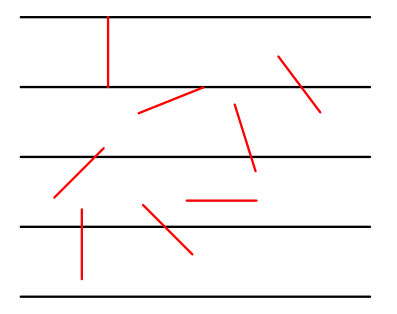
\includegraphics[scale=0.5]{figures/Buffon}
		\end{figure}
	\end{frame}
	
	
	\begin{frame}
		\frametitle{~~蒙特卡洛树搜索算法}
		\text{博弈树搜索算法:将初始状态和所有可能的后续状态通过直接先}
		\text{后关系连接在一起形成博弈树}
		\begin{figure}
			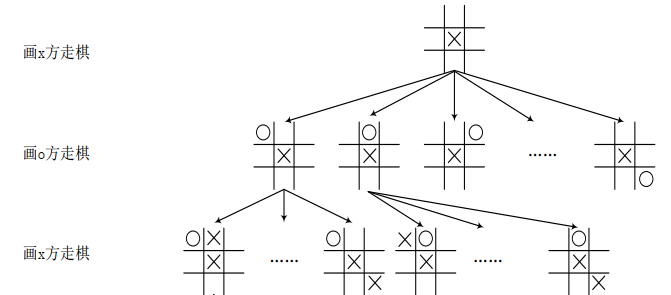
\includegraphics[scale=0.5]{figures/bytree}
		\end{figure}
	\end{frame}
	
	
	\begin{frame}
		\frametitle{~~蒙特卡洛树搜索算法}
		\begin{columns}
			\column<1->{0.5\textwidth}
			\begin{figure}
				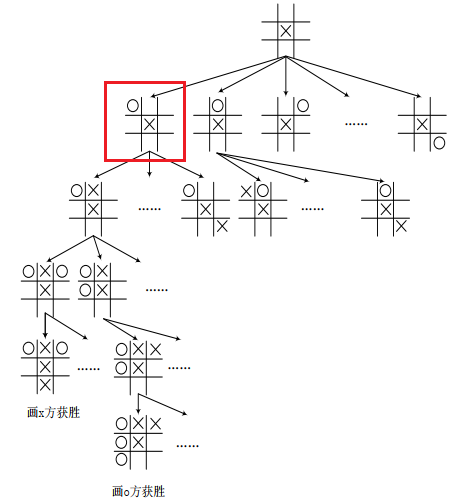
\includegraphics[scale=0.5]{figures/jtree}
			\end{figure}
			
			\column{0.5\textwidth}
			\begin{block}{思想}
				~~~利用经验平均来代替随机变量的期望。如在博弈状态$s$时期望值为$v_{\pi}(s)$,一般难以通过计
				算直接求出该值,但是可以通过蒙特卡洛方法获得一系列收益$G_1(s)$,$\cdots$,$G_n(s)$.根据大数定律,当$n$趋于无穷大时,抽样收益的均值趋近于期望值。定义$v(s)$ 为系列收益的平均值,即
				$$v(s)=\frac{G_1(s)+\cdots+G_n(s)}{n}$$
				\begin{center} 当$n \to \infty$时,$v(s) \rightarrow v_{\pi}(s)$ \end{center}
			\end{block}
		\end{columns}
	\end{frame}
	
	\begin{frame}
		\frametitle{~~蒙特卡洛树搜索算法}
		\Large \text{蒙特卡洛树搜索算法过程} 
		\begin{figure}
			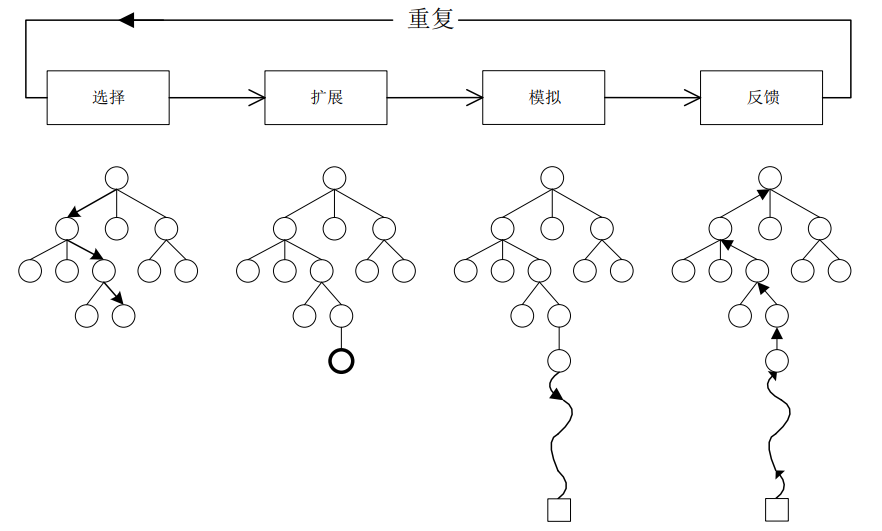
\includegraphics[scale=0.5]{figures/MCTS}
		\end{figure}
	\end{frame}
	
	\subsection*{基于手牌拆分的蒙特卡洛树搜索算法}
	\begin{frame}{~~基于手牌拆分的蒙特卡洛树搜索算法}{~~~~(MCTSHS)}
		\Large \text{基于手牌拆分的蒙特卡洛树搜索算法过程} 
		\begin{figure}
			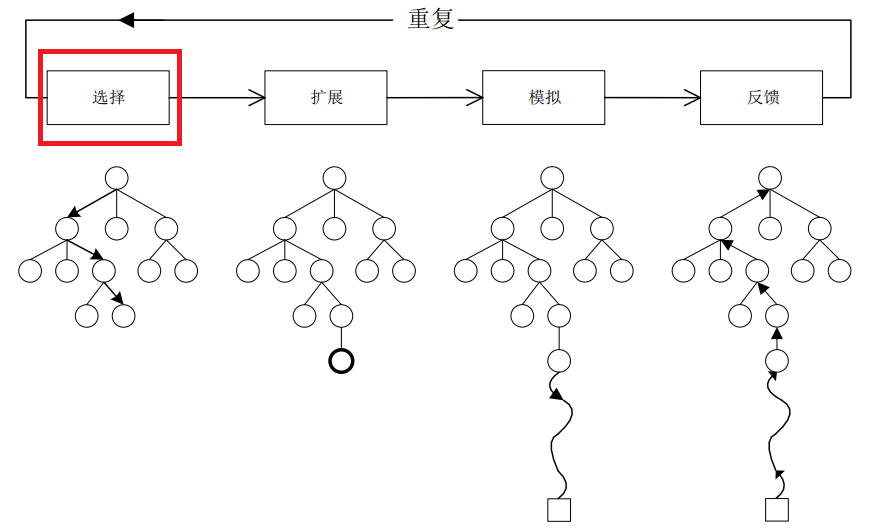
\includegraphics[scale=0.5]{figures/MCTSCF}
		\end{figure}
	\end{frame}
	
	\subsection*{实验比较结果}
	\begin{frame}
		\frametitle{~~与规则算法(RB)比较}
		\begin{block}{规则算法(RB)}
			~~~~该算法分为主动策略和被动策略两种。主动策略中若上轮玩家取得主动权,那本轮该玩家可根据自己手牌主动选择出牌类型,而不需要考虑其他玩家的出牌类型;被动策略中玩家需要考虑本轮其他玩家的出牌, 被动选择跟牌类型。 
		\end{block}
		\text{不区分角色比较结果:}
		\begin{figure}
			\includegraphics<2->[scale=0.4]{figures/AllMvR}
		\end{figure}
	\end{frame}
	
	\begin{frame}
		\frametitle{~~与规则算法(RB)比较}
		\text{地主MCTSHS对农民RB:}
		\begin{figure}
			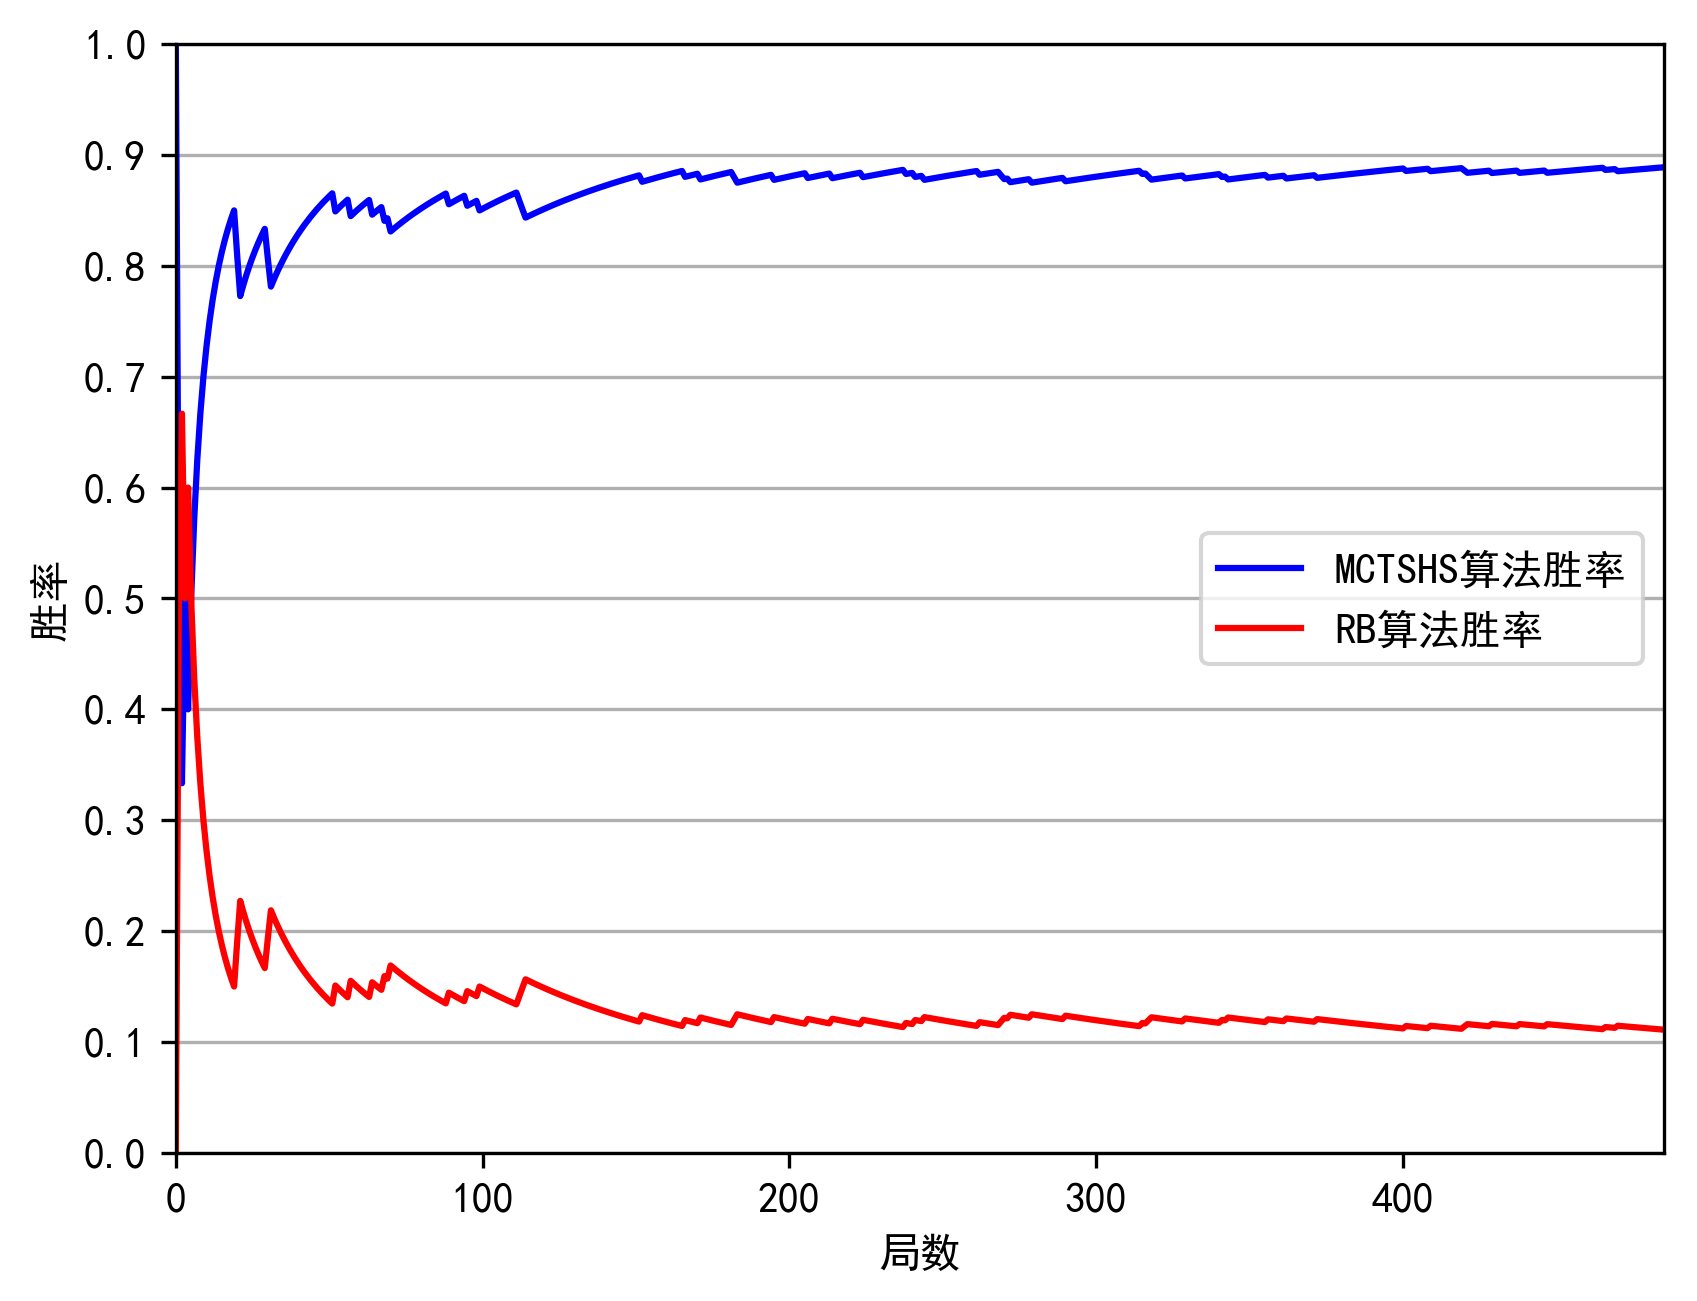
\includegraphics[scale=0.6]{figures/MvR}
		\end{figure}
	\end{frame}
	
	\begin{frame}
		\frametitle{~~与规则算法(RB)比较}
		\text{农民MCTSHS对地主RB:}
		\begin{figure}
			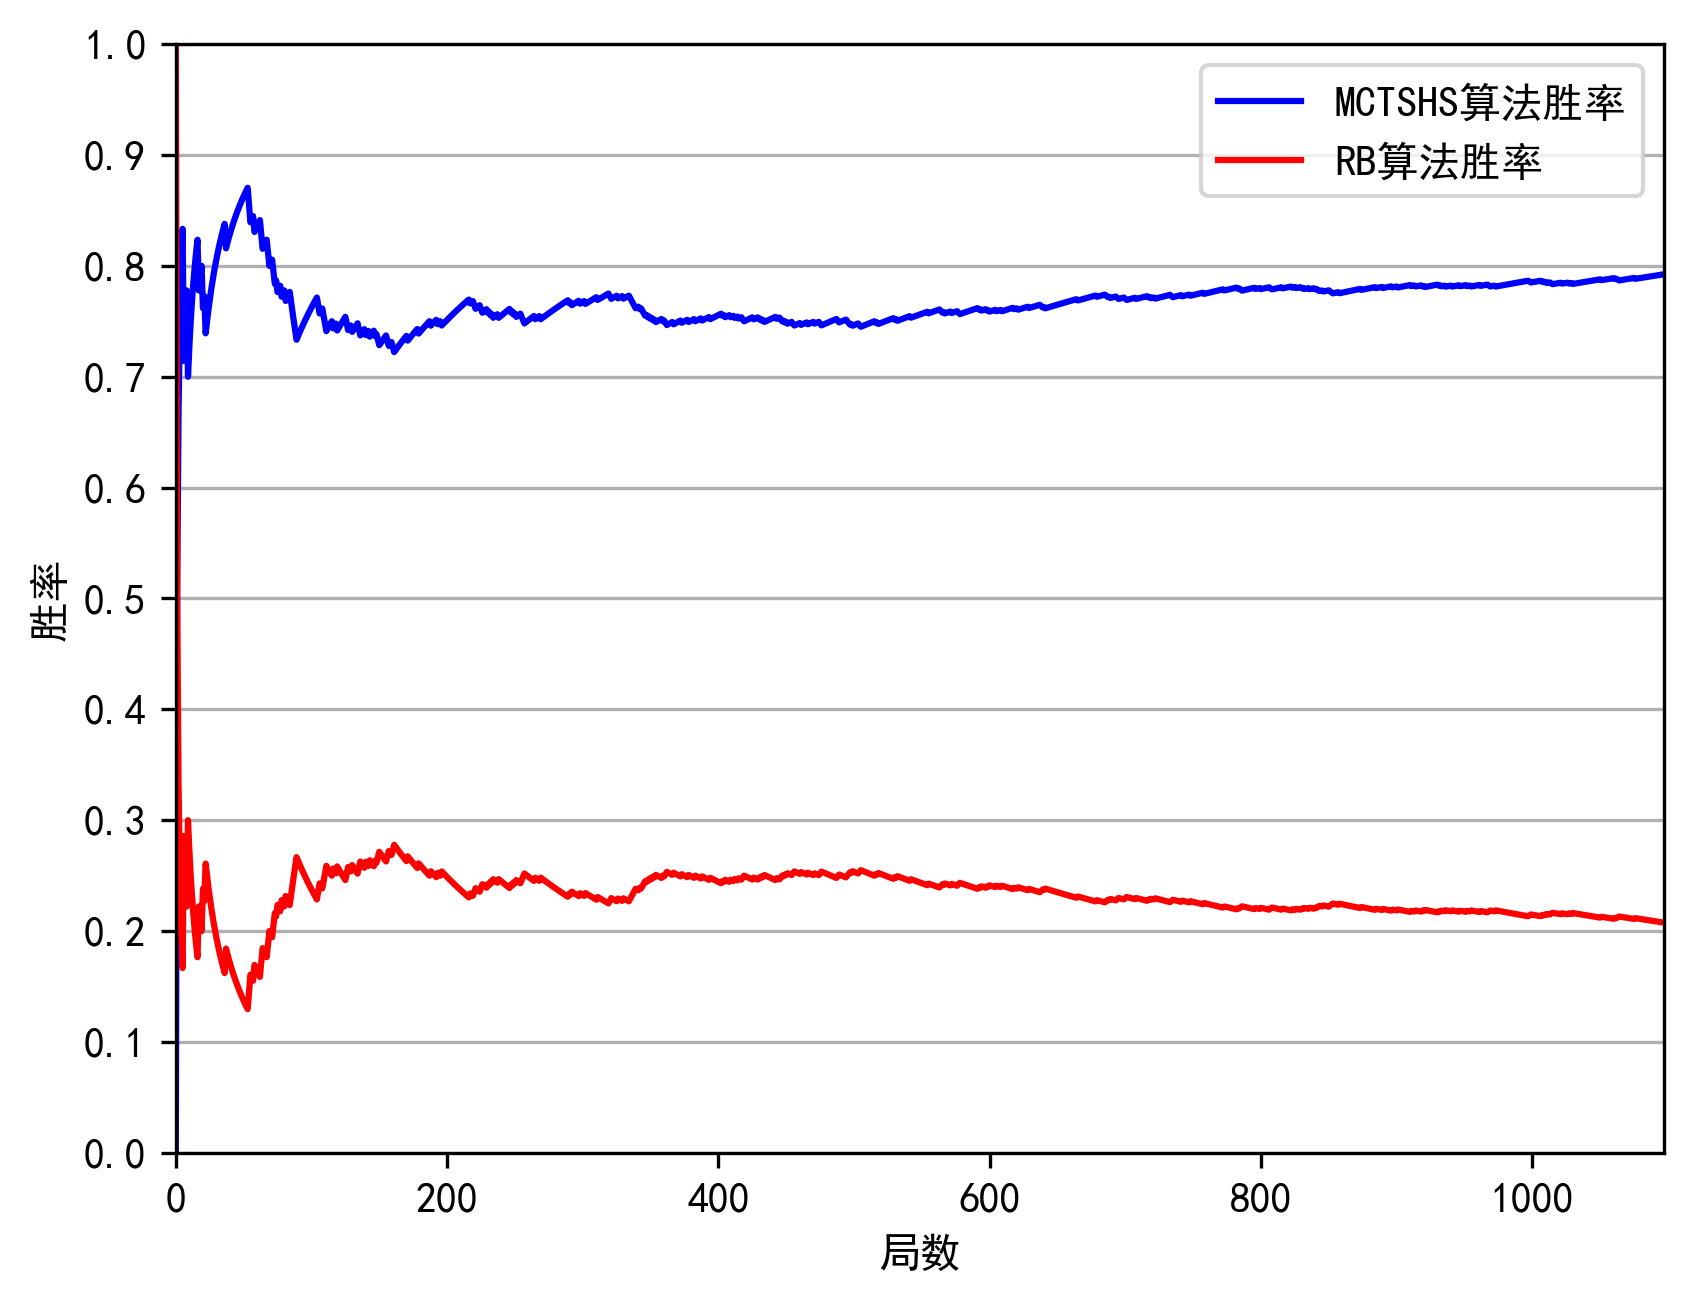
\includegraphics[scale=0.6]{figures/RvM}
		\end{figure}
	\end{frame}
	
	\begin{frame}
		\frametitle{~~与7k7k算法比较}
		\begin{block}{7k7k算法}
			~~~~该算法为北京迦游网络科技有限公司开发的“斗地主”智能算法。 
		\end{block}
		\text{不区分角色比较结果:}
		\begin{figure}
			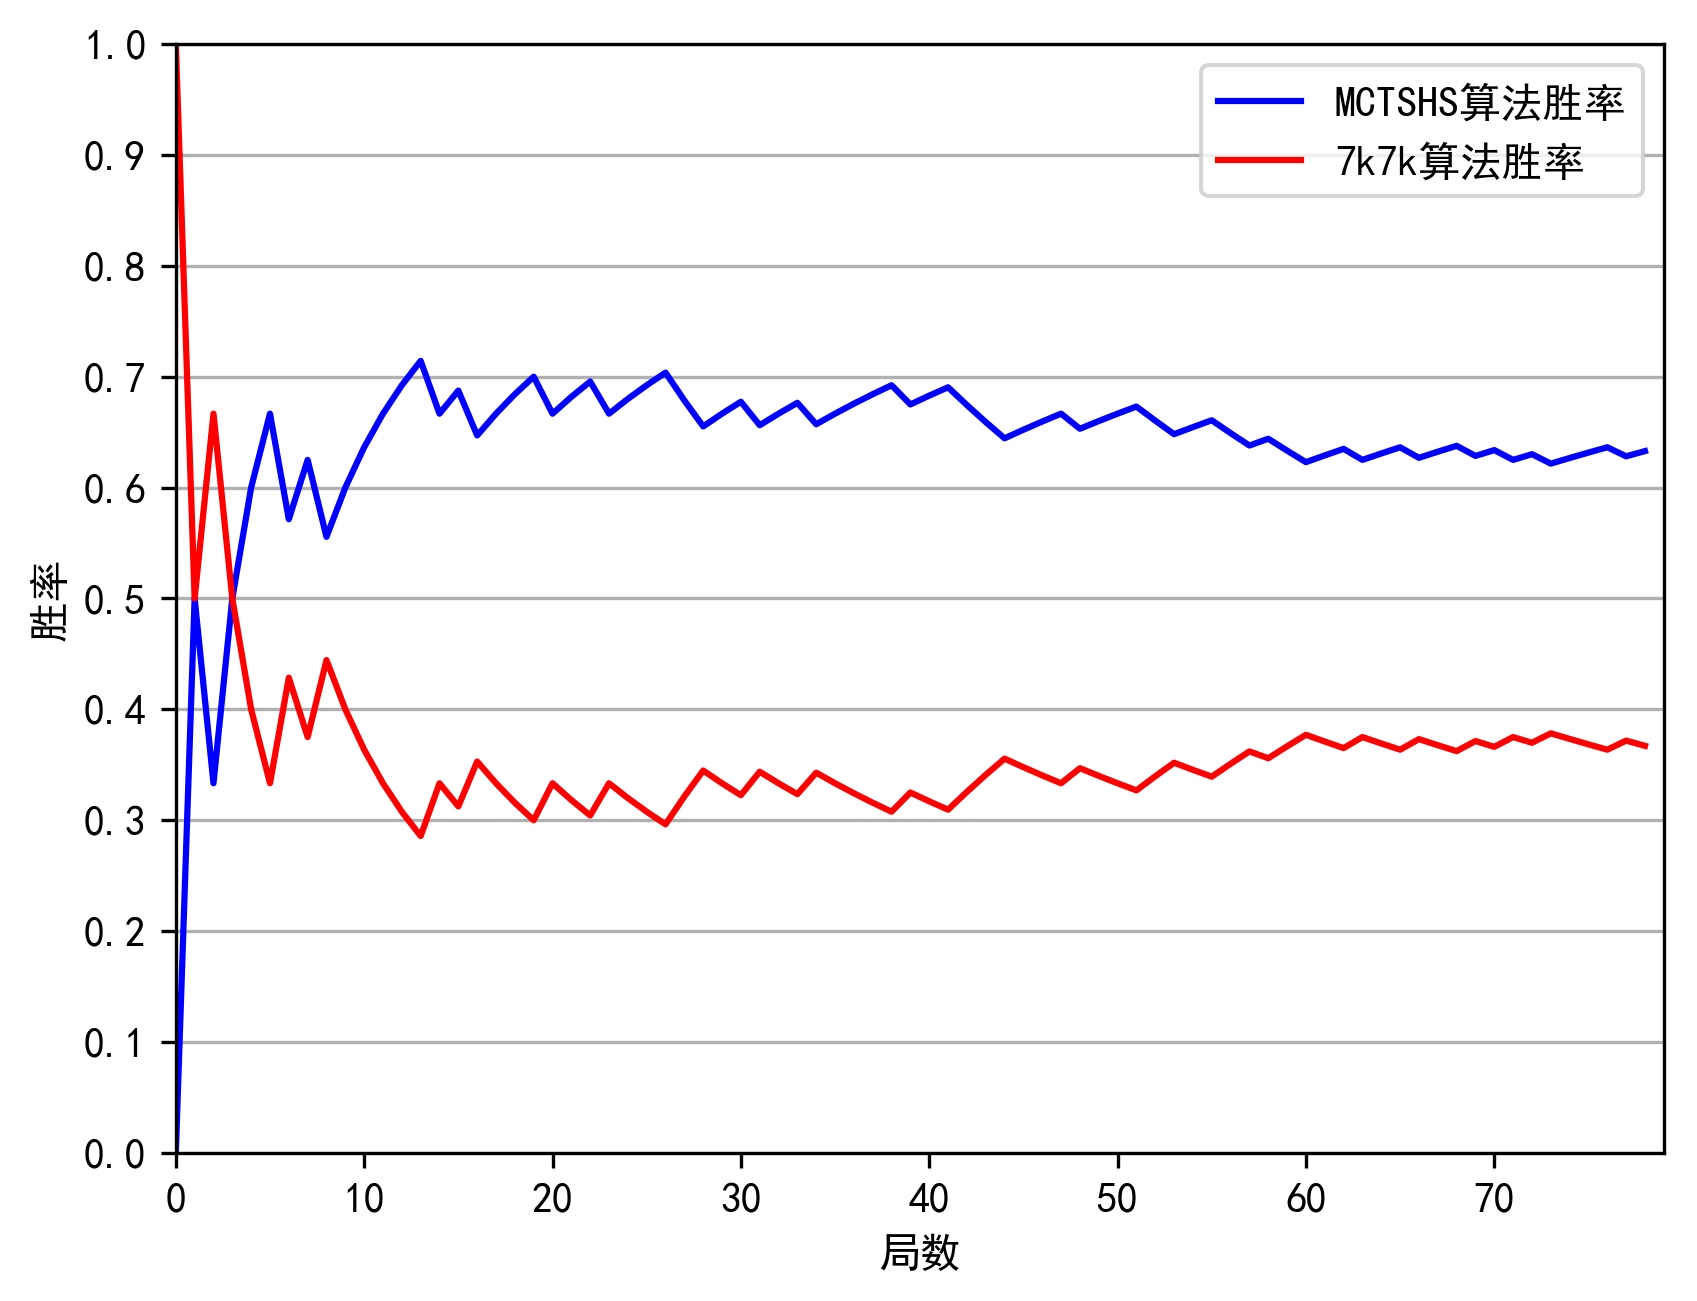
\includegraphics[scale=0.5]{figures/Mv7k7k}
		\end{figure}
	\end{frame}
	
	\subsection*{合作问题分析}
	\begin{frame}
		\frametitle{~~合作问题分析}
		\text{合作问题分析:}
		\begin{figure}
			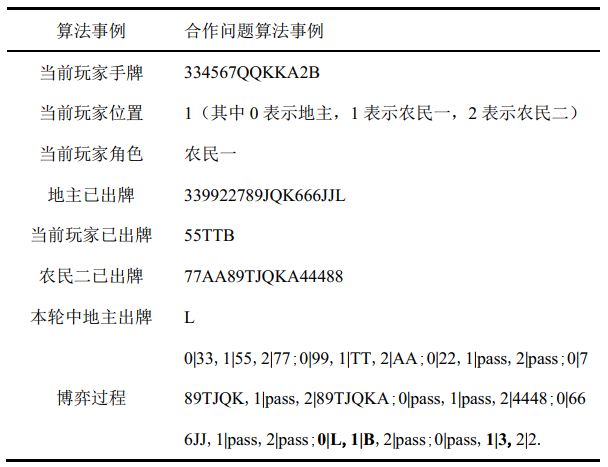
\includegraphics[scale=0.7]{figures/hz}
		\end{figure}
	\end{frame}
	
	\subsection*{算法缺点}
	\begin{frame}
		\frametitle{~~算法缺点}
		\begin{spacing}{2.0}
			\text{算法缺点:}
			\begin{itemize}
				\item 每次决策思考时间过长
				\item 已搜索到的决策未能充分利用
			\end{itemize}
		\end{spacing}
	\end{frame}
	
	\begin{frame}
		\frametitle{~~算法缺点}
		\begin{spacing}{2.0}
			\text{算法缺点:}
			\begin{itemize}
				\item<1-> 每次决策思考时间过长
				\item<1-> 已搜索到的决策未能充分利用
			\end{itemize}
		\end{spacing}
		\LARGE \text{{\LARGE 改进算法!!}}
	\end{frame}
	
	\section{结合卷积神经网络的蒙特卡洛树搜索}
	\subsection*{结合卷积神经网络的蒙特卡洛树搜索}
	\begin{frame}
		\frametitle{~结合卷积神经网络的蒙特卡洛树搜索模型MCM}
		\[
		\text{{\Large \textbf{MCM模型}}}
		\begin{cases}
			\text{手牌拆分的蒙特卡洛树搜索模块} \\ \\
			\text{CNN策略学习模块}\\ \\
			\text{改善策略模块}
		\end{cases}
		\]
		\large \text{CNN策略学习模块:} 
		\begin{figure}
			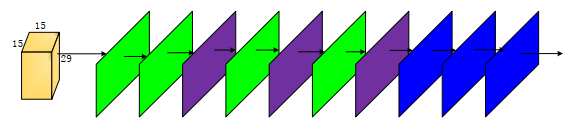
\includegraphics[scale=0.85]{figures/cnn}
		\end{figure}
	\end{frame}
	
	\begin{frame}
		\frametitle{~结合卷积神经网络的蒙特卡洛树搜索模型MCM}
		\[
		\text{{\Large \textbf{MCM模型}}}
		\begin{cases}
			\text{手牌拆分的蒙特卡洛树搜索模块} \\ \\
			\text{CNN策略学习模块}\\ \\
			\text{改善策略模块}
		\end{cases}
		\]
		\large \text{CNN策略学习模块:} 
		\begin{figure}
			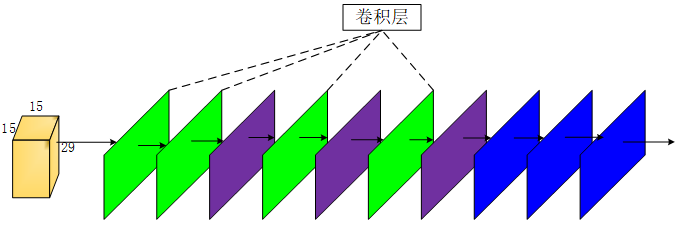
\includegraphics[scale=0.65]{figures/cnn1}
		\end{figure}
	\end{frame}
	
	\begin{frame}
		\frametitle{~结合卷积神经网络的蒙特卡洛树搜索模型MCM}
		\[
		\text{{\Large \textbf{MCM模型}}}
		\begin{cases}
			\text{手牌拆分的蒙特卡洛树搜索模块} \\ \\
			\text{CNN策略学习模块}\\ \\
			\text{改善策略模块}
		\end{cases}
		\]
		\large \text{CNN策略学习模块:} 
		\begin{figure}
			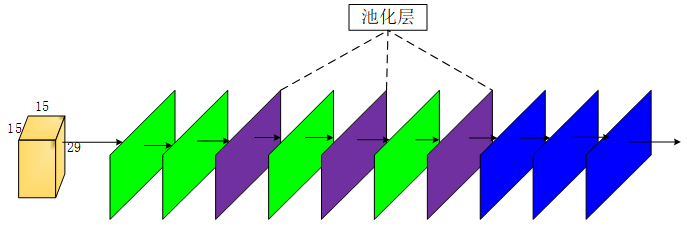
\includegraphics[scale=0.65]{figures/cnn2}
		\end{figure}
	\end{frame}
	
	\begin{frame}
		\frametitle{~结合卷积神经网络的蒙特卡洛树搜索模型MCM}
		\[
		\text{{\Large \textbf{MCM模型}}}
		\begin{cases}
			\text{手牌拆分的蒙特卡洛树搜索模块} \\ \\
			\text{CNN策略学习模块}\\ \\
			\text{改善策略模块}
		\end{cases}
		\]
		\large \text{CNN策略学习模块:} 
		\begin{figure}
			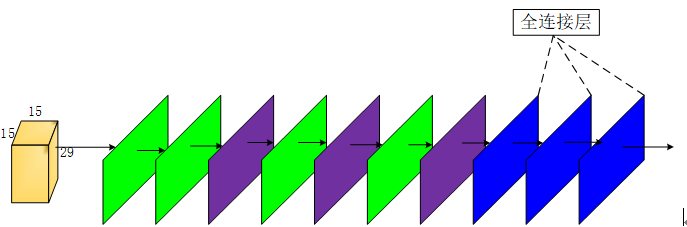
\includegraphics[scale=0.65]{figures/cnn3}
		\end{figure}
	\end{frame}
	
	\begin{frame}
		\frametitle{~结合卷积神经网络的蒙特卡洛树搜索模型MCM}
		\[
		\text{{\Large \textbf{MCM模型}}}
		\begin{cases}
			\text{手牌拆分的蒙特卡洛树搜索模块} \\ \\
			\text{CNN策略学习模块}\\ \\
			\text{改善策略模块}
		\end{cases}
		\]
		\large \text{CNN策略学习模块:} 
		\begin{figure}
			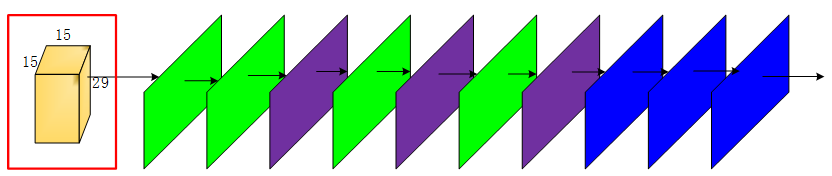
\includegraphics[scale=0.55]{figures/cnnInput}
		\end{figure}
	\end{frame}
	
	\subsection*{CNN策略学习模块}
	\begin{frame}
		\frametitle{~~CNN策略学习模块-----输入表示}
		\begin{itemize}
			\item<1-> X维度:表示15种扑克
			\item<2-> Y维度:
			\begin{itemize}
				\item<3-> 0-3(下标)表示扑克的张数
				\item<4-> 4-13(下标)表示扑克是否参与组成出牌类型
				\item<5-> 14(下标)表示该出牌是否为地主玩家。
			\end{itemize}
			\item<6-> Z维度:\vspace{-0.05cm}\begin{figure}
				\includegraphics<6->[scale=0.6]{figures/z}
			\end{figure}
		\end{itemize}
	\end{frame}
	
	\begin{frame}
		\frametitle{~~CNN策略学习模块}
		\begin{spacing}{2.0}
			\begin{itemize}
				\item 学习样本处理
				\begin{itemize}
					\item 将MCTSHS决策结果的数据进行去重
					\item 随机打乱去重后的样本顺序,并从打乱的样本中,随机选择 90\%的样本组成训练集, 10\%作为测试集
				\end{itemize}
			\end{itemize}
		\end{spacing}
	\end{frame}
	
	\begin{frame}
		\frametitle{~~CNN策略学习模块}
		\begin{spacing}{1.5}
			\begin{itemize}
				\item<1-> 学习样本处理
				\begin{itemize}
					\item<1-> 将MCTSHS决策结果的数据进行去重
					\item<1-> 随机打乱去重后的样本顺序,并从打乱的样本中,随机选择 90\%的样本组成训练集, 10\%作为测试集
				\end{itemize}
			\end{itemize}
		\end{spacing}
		\text{\textbf{MCTSHS学习的部分历史数据记录:}}
		\begin{figure}
			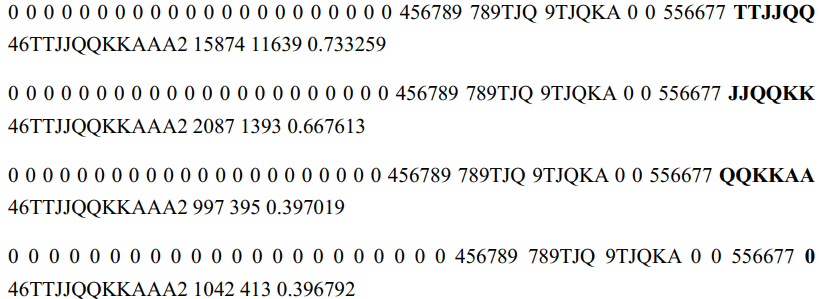
\includegraphics[scale=0.35]{figures/sample}
		\end{figure}
	\end{frame}
	
	\begin{frame}
		\frametitle{~~CNN策略学习模块}
		\text{CNN网络学习策略损失变化图:}
		\begin{figure}
			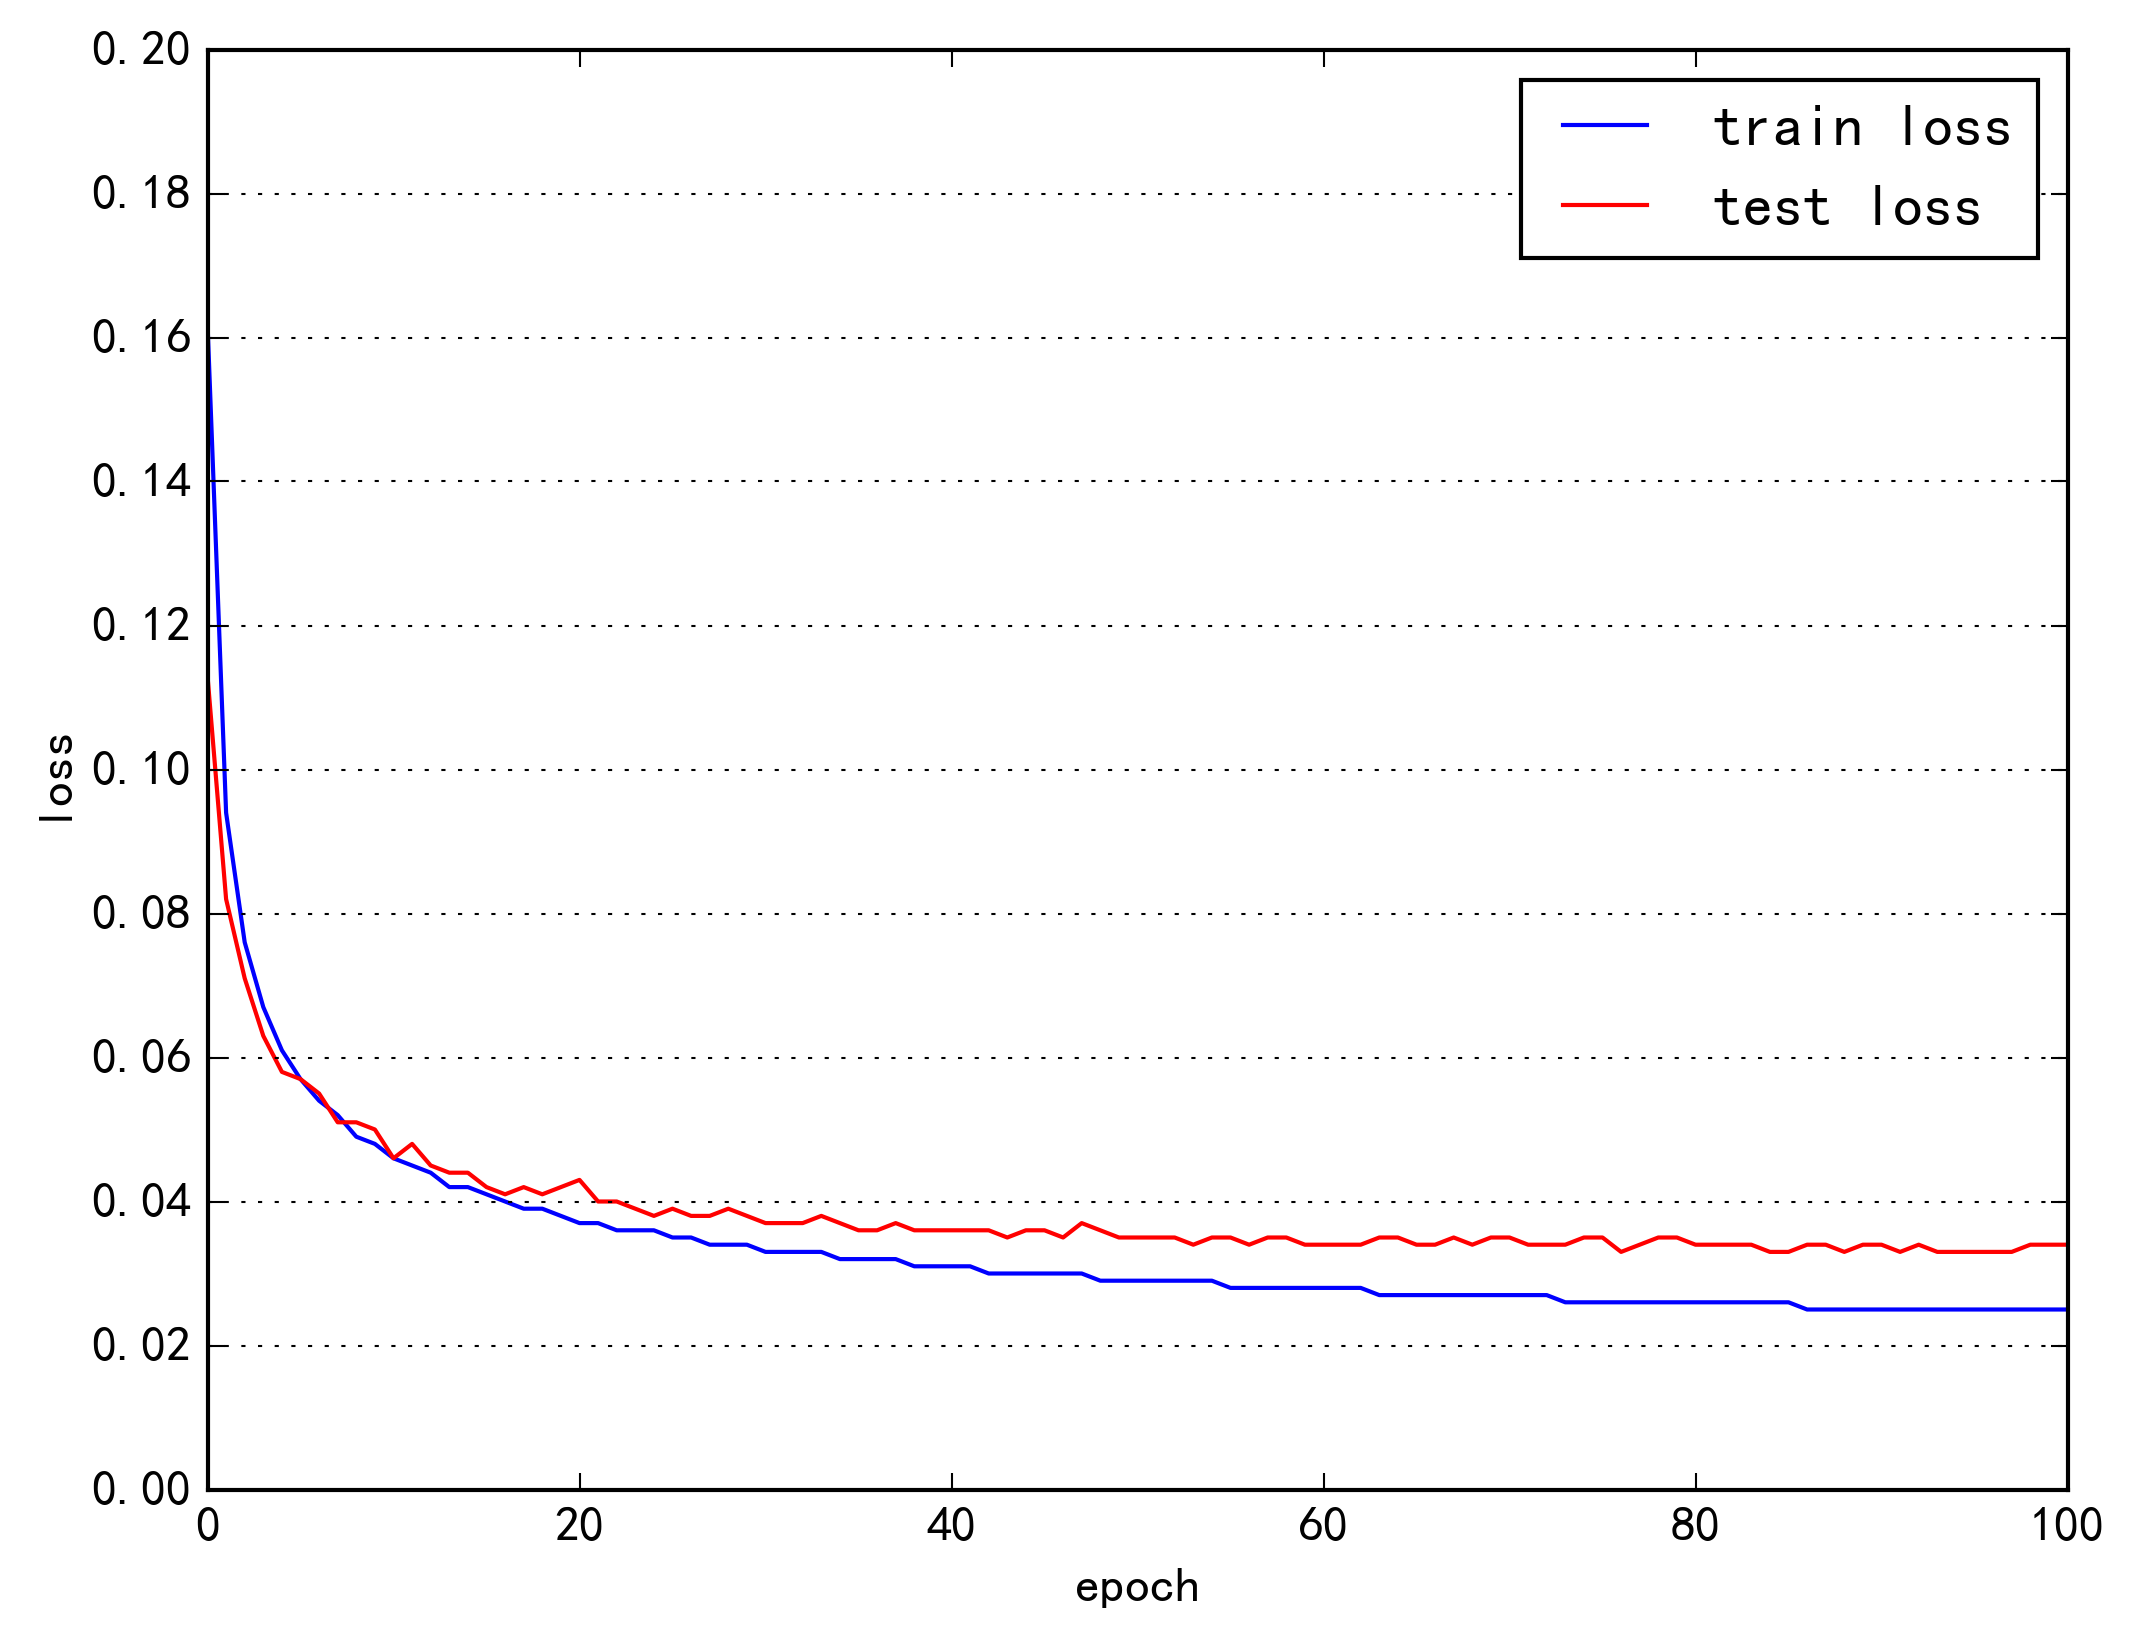
\includegraphics[scale=0.5]{figures/loss}
		\end{figure}
	\end{frame}
	
	\subsection*{实验结果}
	\begin{frame}
		\frametitle{~~实验结果-----实验比较设定}
		\text{实验比较设定}
		\begin{itemize}
			\item 地主、农民使用不同的决策算法,其中农民一、农民二均使用农民的决策算法
			\item 地主、农民一、农民二使用不同的决策算法
			\item 地主、农民一、农民二使用不同的决策算法进行相同牌局比较
		\end{itemize}
	\end{frame}
	
	\begin{frame}
		\frametitle{~~实验结果-----与随机算法(Random)比较}
		\begin{block}{随机算法(Random)介绍}
			~~~~思路为:根据玩家的手牌、 本轮其它玩家出牌等信息按照博弈规则计算出当前状态下玩家可能的所有出牌, 并从中随机选择一种可能出牌作为本轮的最终出牌。
		\end{block}
		\text{地主 MCM 对农民 Random 的胜率变化图:}\vspace{-0.1cm}
		\begin{figure}
			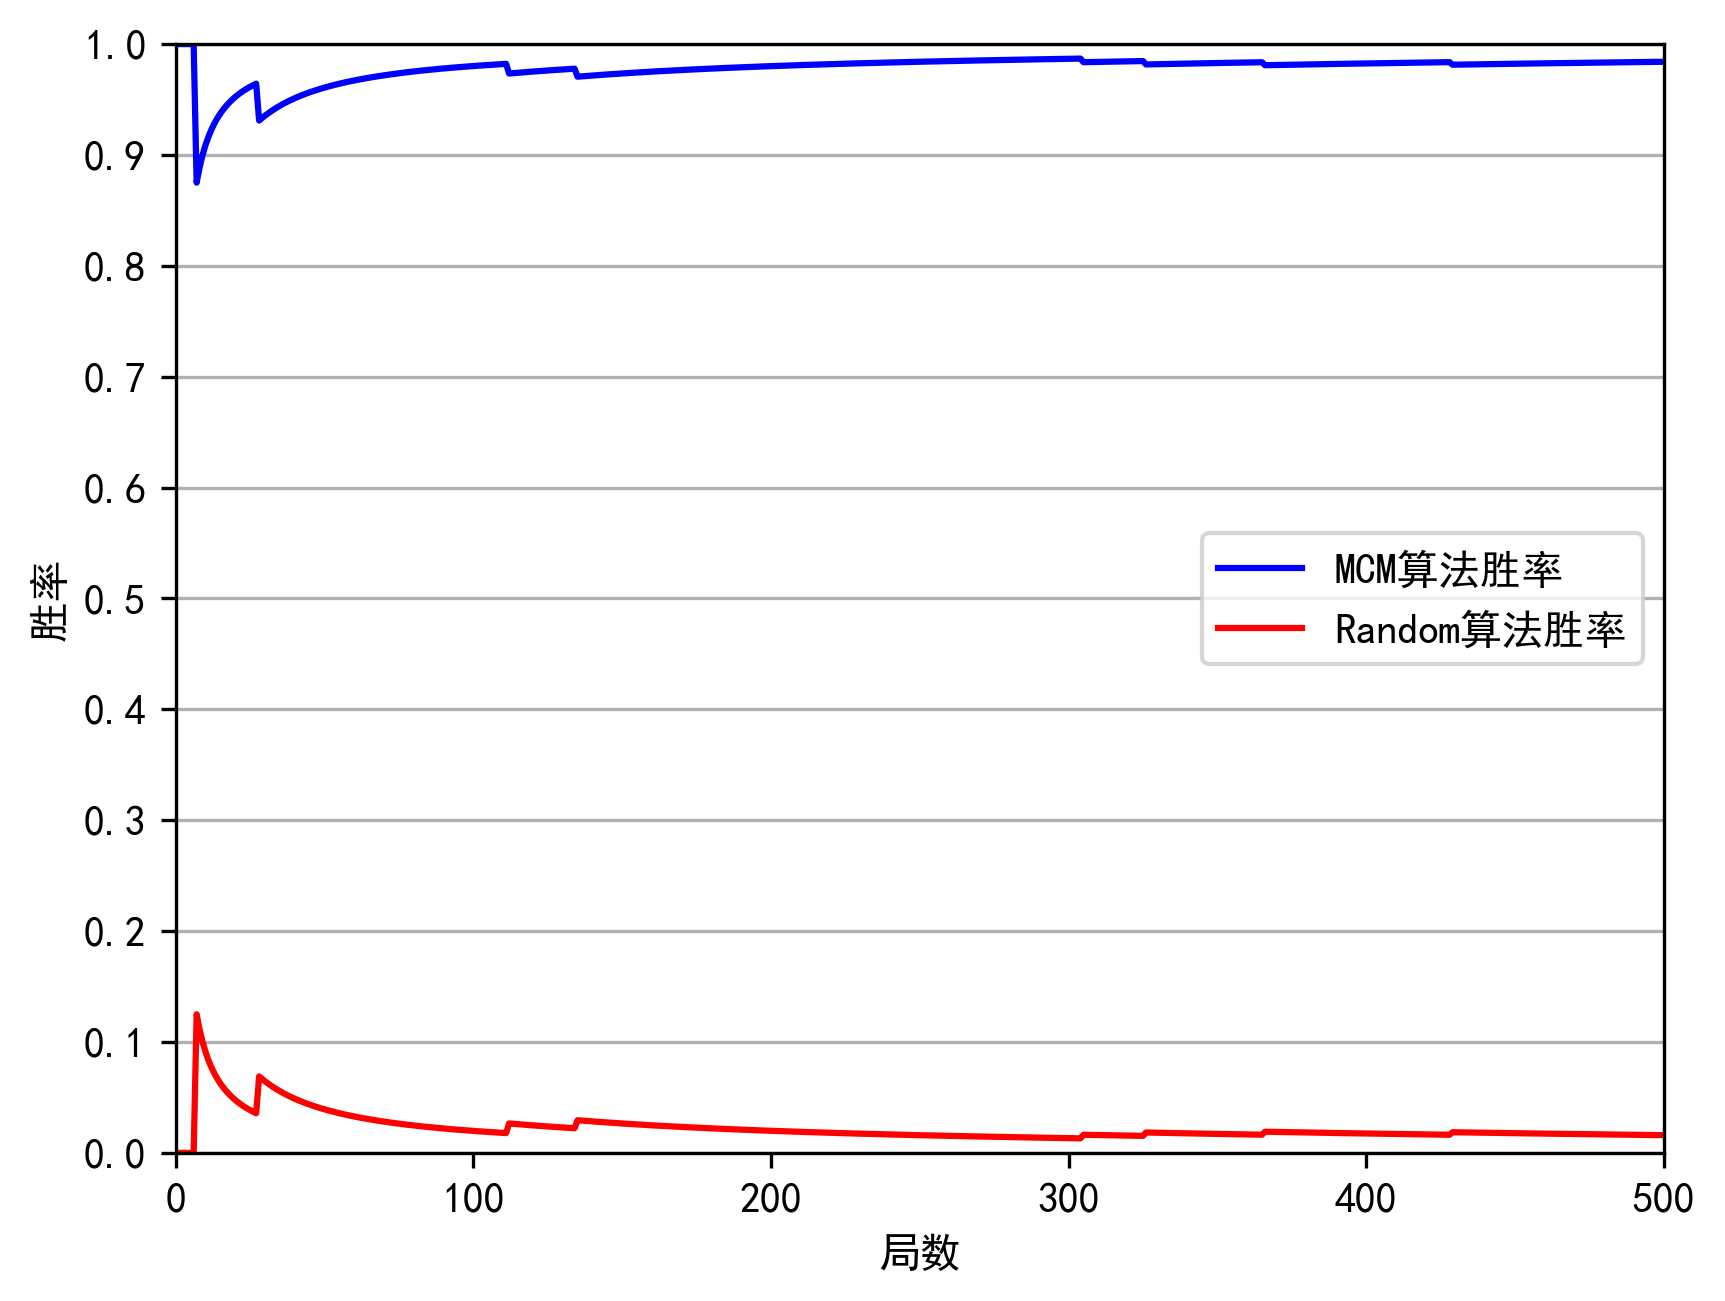
\includegraphics[scale=0.45]{figures/MCvR}
		\end{figure}
	\end{frame}
	
	\begin{frame}
		\frametitle{~~实验结果-----与随机算法(Random)比较}
		\text{农民MCM 对地主Random 的胜率变化图:}\vspace{-0.1cm}
		\begin{figure}
			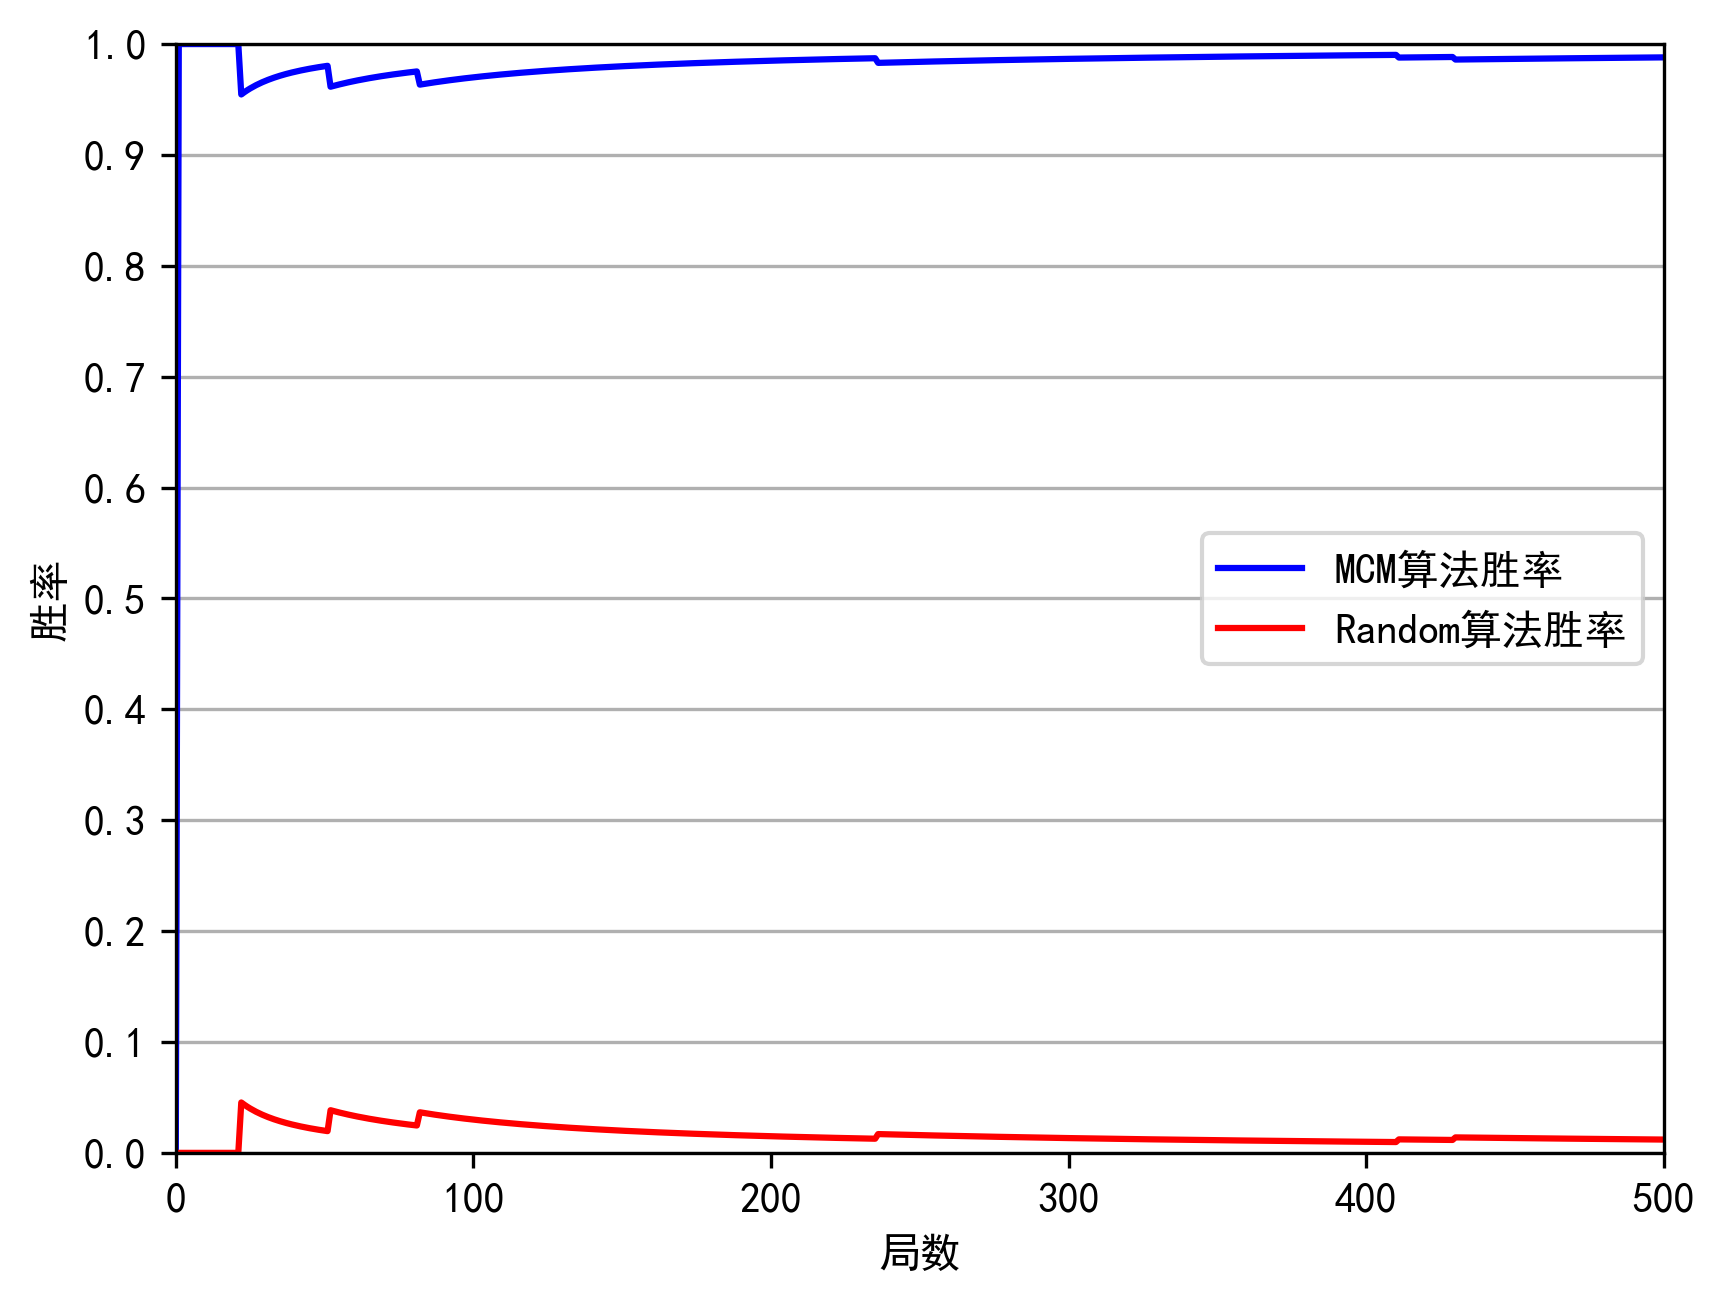
\includegraphics[scale=0.6]{figures/RvMC}
		\end{figure}
	\end{frame}
	
	
	\begin{frame}
		\frametitle{~~实验结果-----与RHCP算法比较}
		\begin{block}{RHCP算法介绍}
			~~~~该算法引入手牌剩余价值的概念,其总体思路是将手牌按照“斗地主”规则进行不同的组合,并选择使得出牌后手牌价值较高的出牌作为本轮最佳出牌。
		\end{block}
		\text{地主 MCM 对农民 RHCP 的胜率变化图:}\vspace{-0.1cm}
		\begin{figure}
			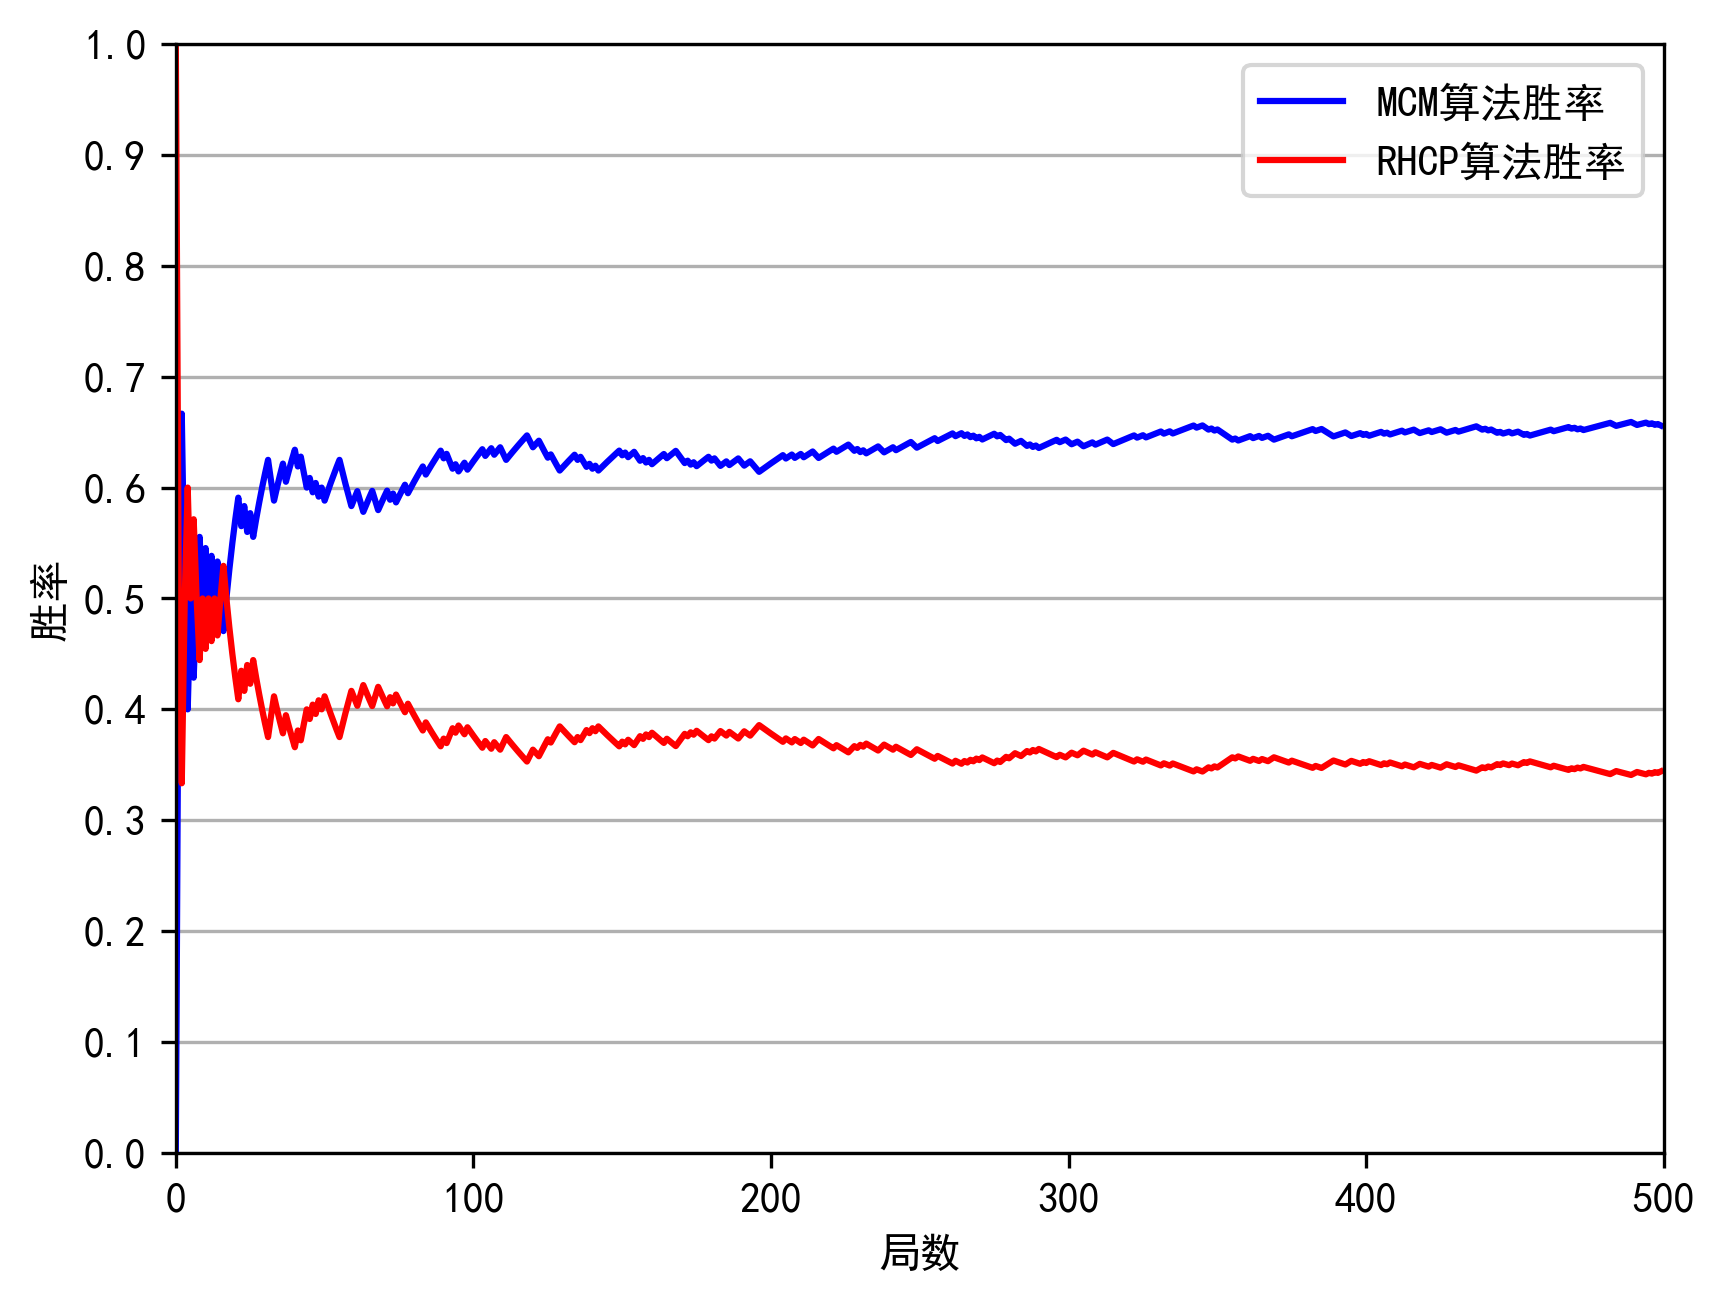
\includegraphics[scale=0.45]{figures/MCvRHCP}
		\end{figure}
	\end{frame}
	
	\begin{frame}
		\frametitle{~~实验结果-----与RHCP算法比较}
		\text{农民MCM 对地主RHCP 的胜率变化图:}\vspace{-0.1cm}
		\begin{figure}
			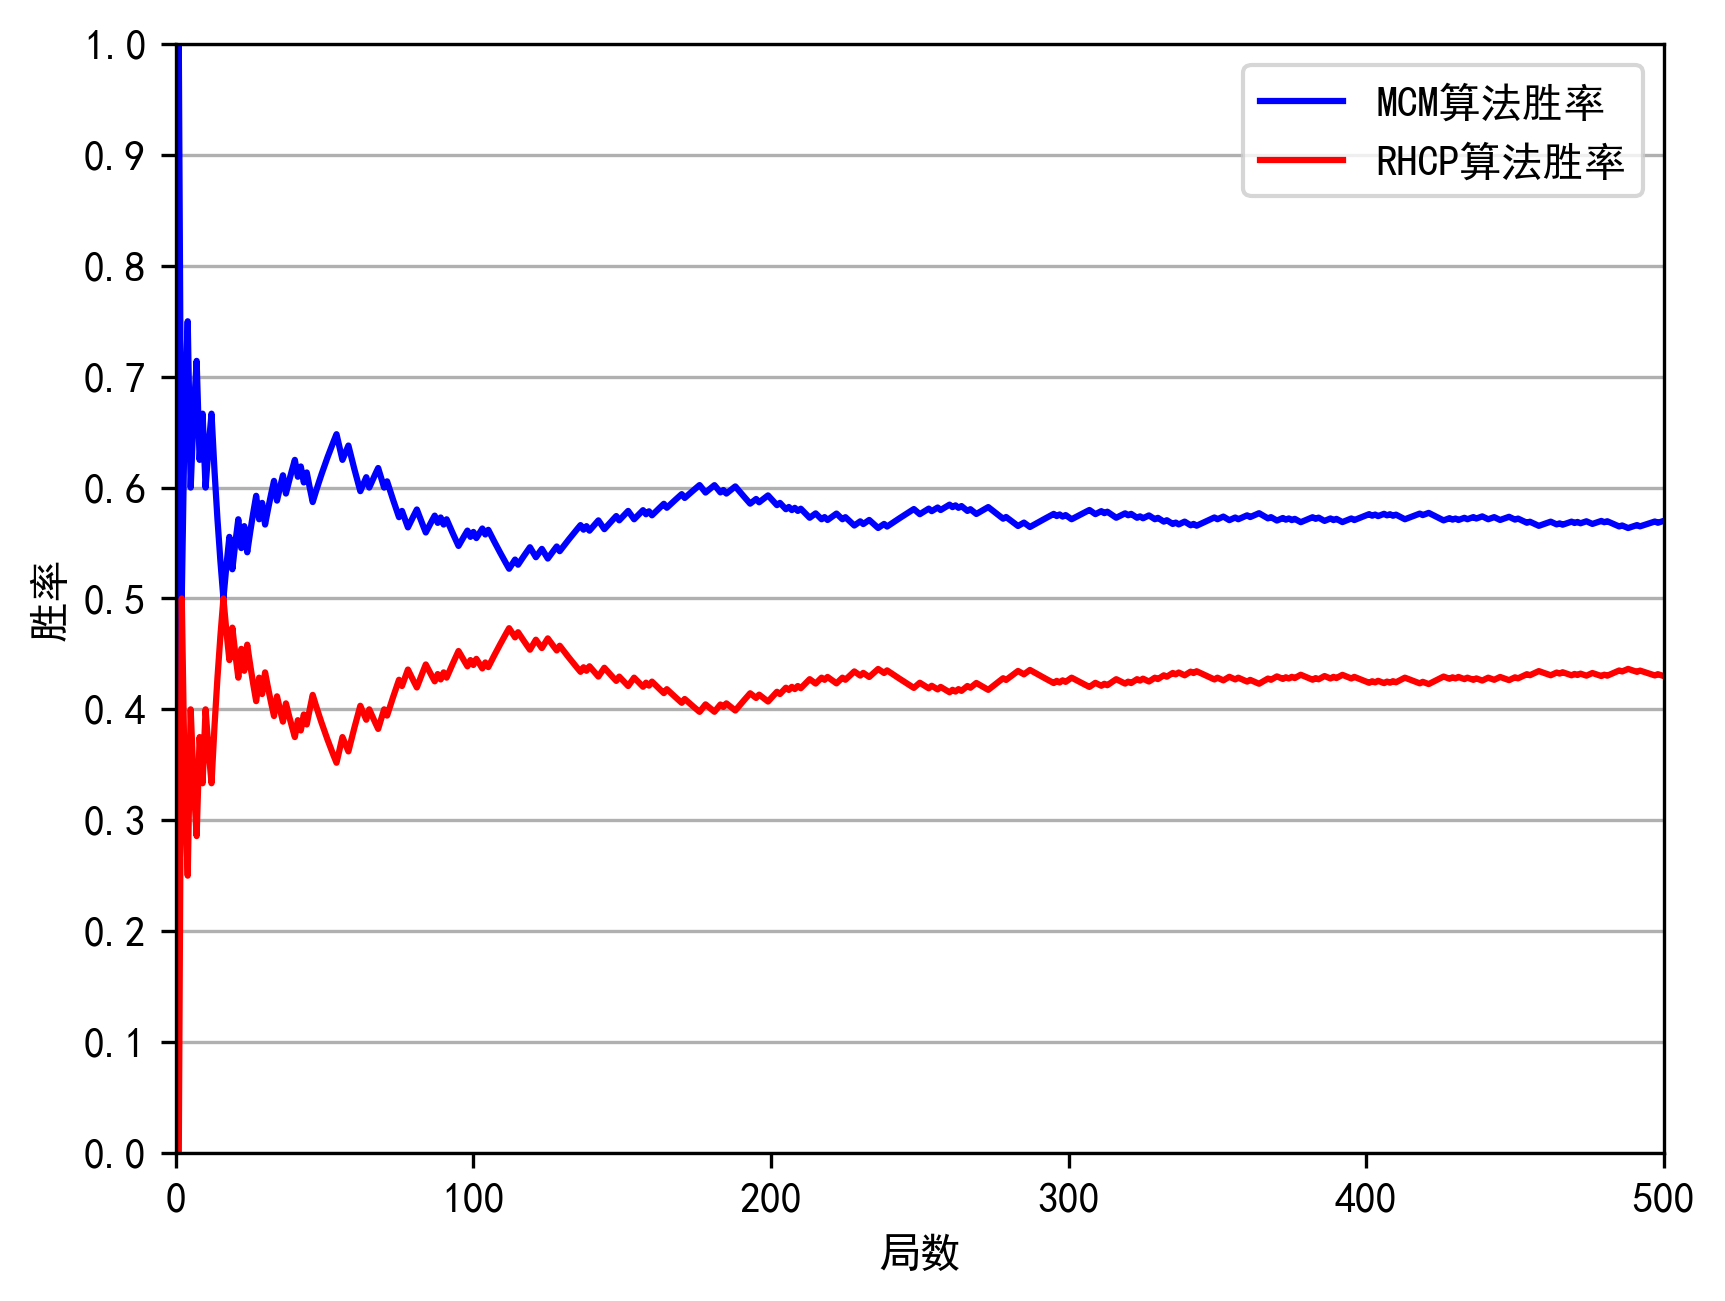
\includegraphics[scale=0.6]{figures/RHCPvMC}
		\end{figure}
	\end{frame}
	
	\begin{frame}
		\frametitle{~~实验结果-----与CQL算法比较}
		\begin{block}{CQL算法介绍}
			~~~~该算法由上海交通大学 You Y 等人提出。You Y 等人针对“斗地主” 博弈中, 每次出牌时存在较多可能组合牌型的情况,提出一种处理组合动作的新方法组合Q学习(CQL)。 
		\end{block}
		\text{地主 MCM 对农民 CQL 的胜率变化图:}\vspace{-0.1cm}
		\begin{figure}
			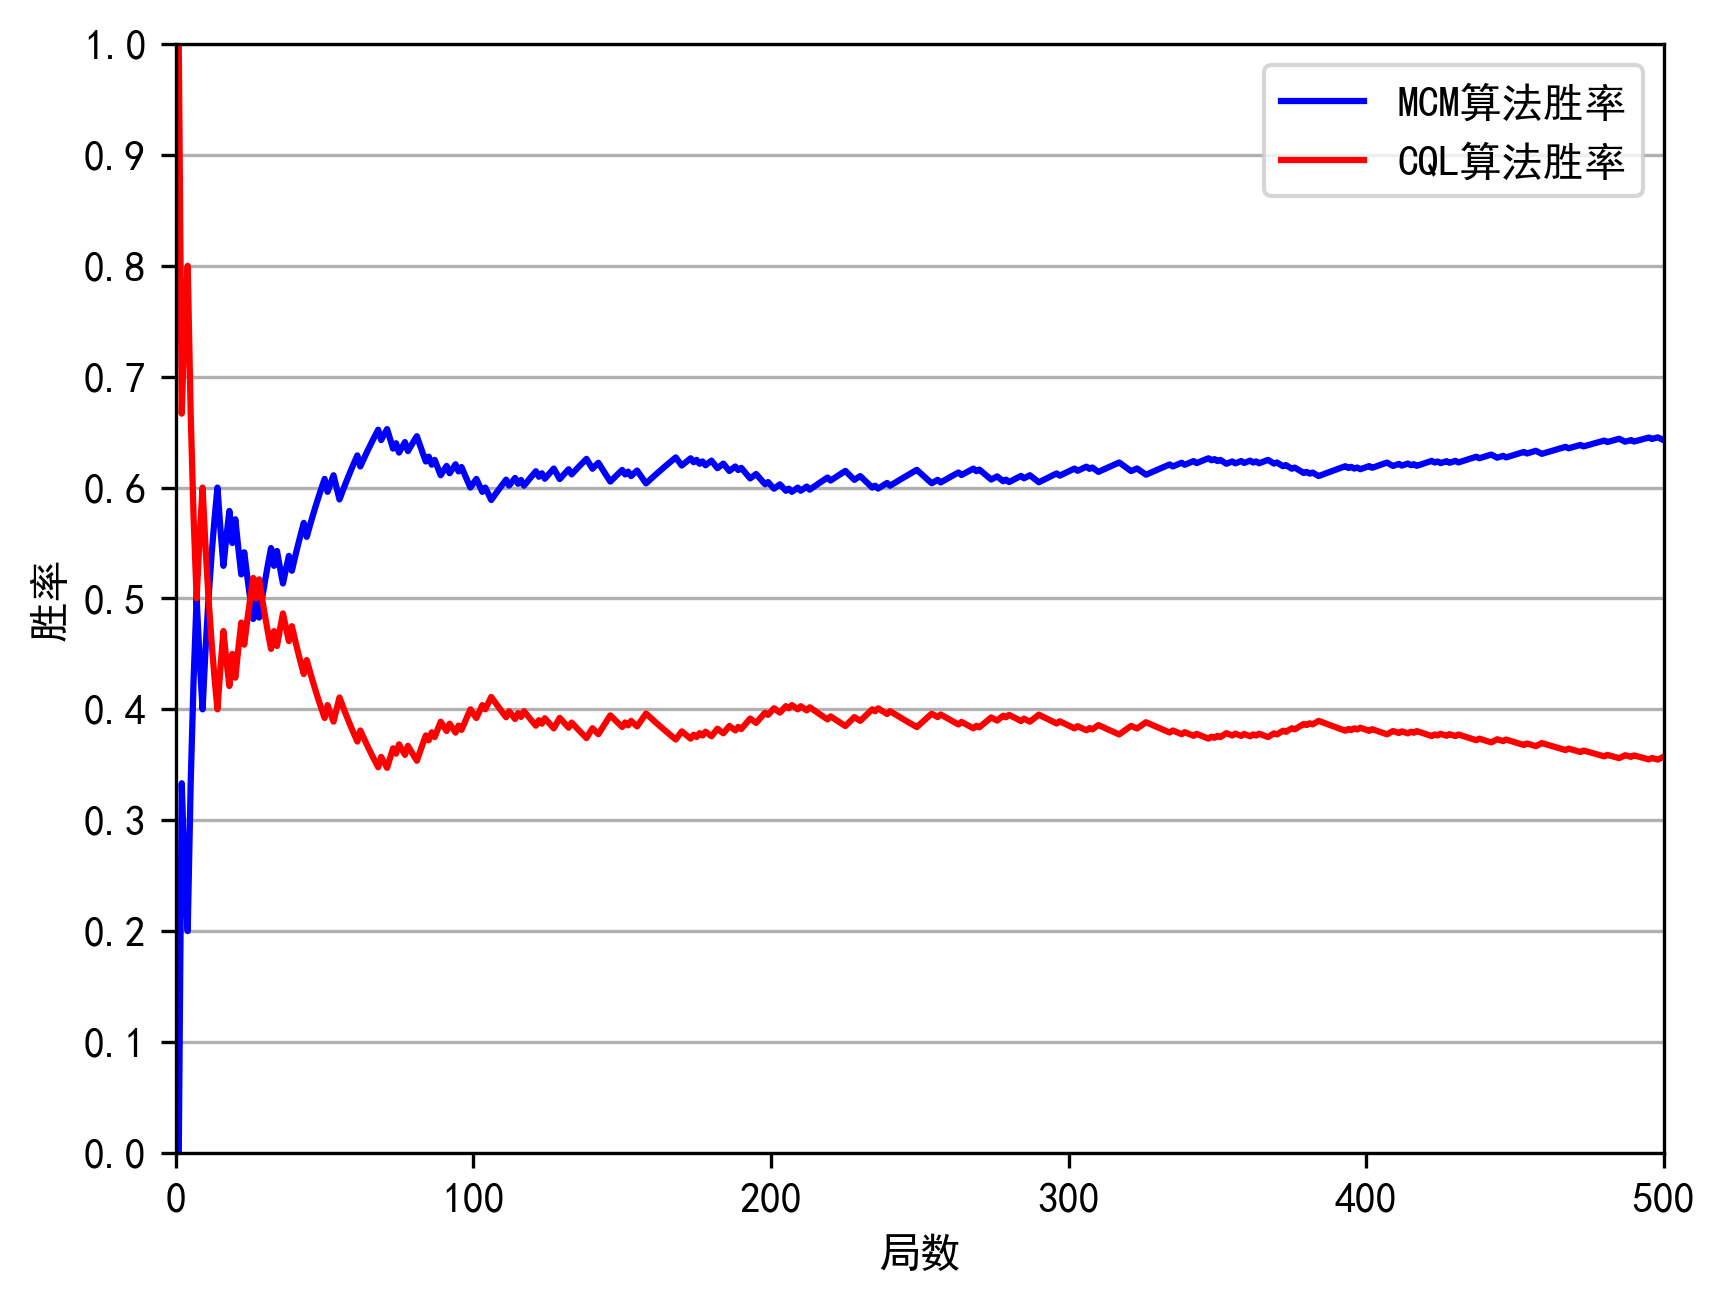
\includegraphics[scale=0.45]{figures/MvC}
		\end{figure}
	\end{frame}
	
	\begin{frame}
		\frametitle{~~实验结果-----与CQL算法比较}
		\text{农民MCM 对地主CQL 的胜率变化图:}\vspace{-0.1cm}
		\begin{figure}
			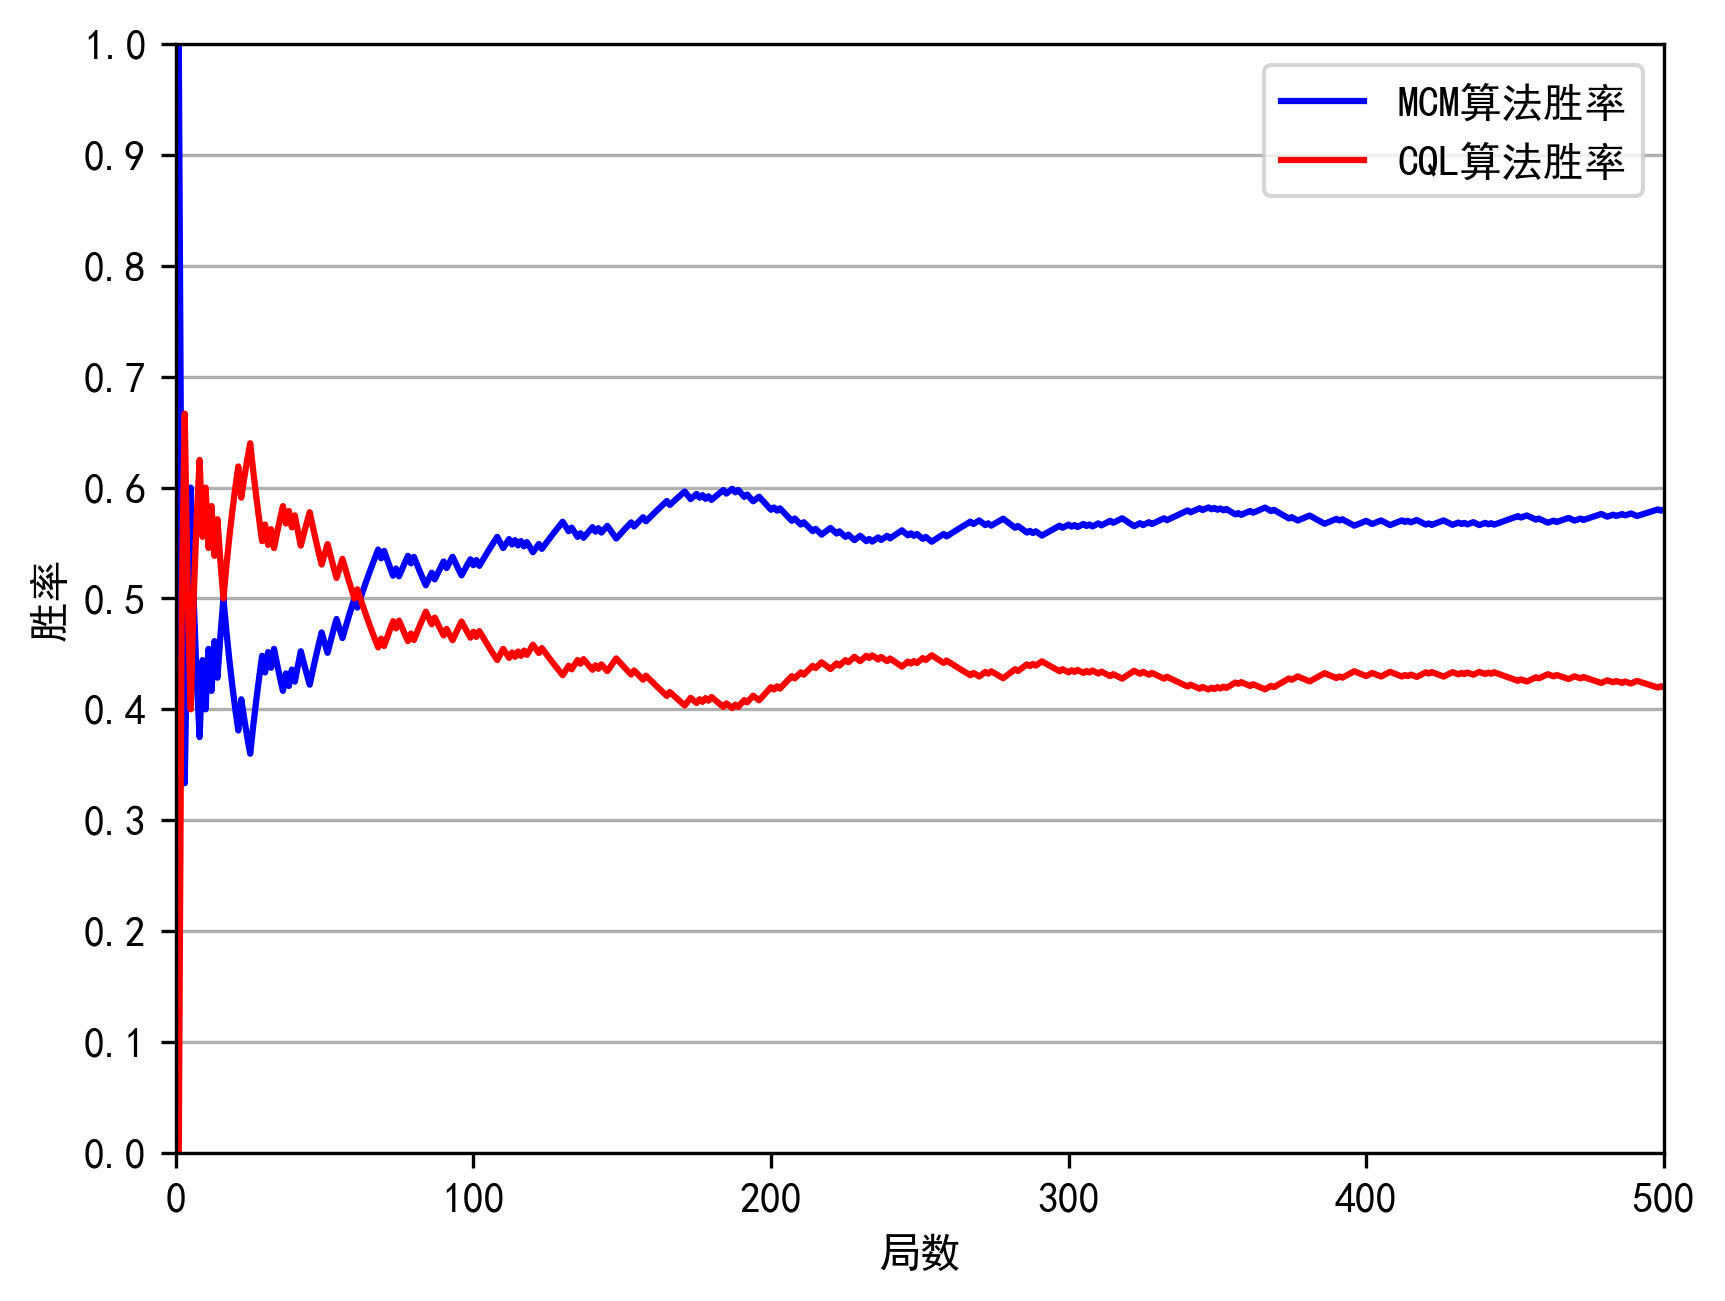
\includegraphics[scale=0.6]{figures/CvM}
		\end{figure}
	\end{frame}
	
	\begin{frame}
		\frametitle{~~实验结果-----CQL、RHCP、MCM相互比较}
		\text{CQL、RHCP以及MCM算法相互比较:}
		\begin{center}
			\begin{tabular}{|c|c|c|c|c|c|}
				\hline 
				\multicolumn{2}{|c|}{地主} & \multicolumn{2}{|c|}{农民一} &  \multicolumn{2}{|c|}{农民二}  \\ 
				\hline 
				决策算法 & 胜率 & 决策算法 & 胜率 & 决策算法 & 胜率 \\ 
				\hline 
				CQL & 44.4\% & RHCP & 21.6\% & MCM & 34\% \\ 
				\hline 
				CQL & 44.8\% & MCM & 21.6\% & RHCP & 33.6\% \\ 
				\hline 
				RHCP & 52.6\% & CQL & 6.4\% & MCM & 41\% \\ 
				\hline 
				RHCP & 46.4\% & MCM & 28\% & CQL & 25.6\% \\ 
				\hline 
				MCM & 63\% & CQL & 6\% & RHCP & 31\% \\ 
				\hline 
				MCM & 59.2\% & RHCP & 26.6\% & CQL & 14.2\% \\ 
				\hline 
				MCM & 56\% & MCM & 22.4\% & MCM & 21.6\% \\ 
				\hline 
			\end{tabular} 
		\end{center}
	\end{frame}
	
	\begin{frame}
		\frametitle{~~实验结果-----CQL、RHCP、MCM相互比较}
		\text{CQL、RHCP以及MCM算法相互比较:}
		\begin{center}
			\begin{tabular}{|c|c|c|c|c|c|}
				\hline 
				\multicolumn{2}{|c|}{地主} & \multicolumn{2}{|c|}{农民一} &  \multicolumn{2}{|c|}{农民二}  \\ 
				\hline 
				决策算法 & 胜率 & 决策算法 & 胜率 & 决策算法 & 胜率 \\ 
				\hline 
				CQL & 44.4\% & RHCP & 21.6\% & MCM & 34\% \\ 
				\hline 
				CQL & 44.8\% & MCM & 21.6\% & RHCP & 33.6\% \\ 
				\hline 
				RHCP & 52.6\% & CQL & 6.4\% & MCM & \multicolumn{1}{>{\columncolor{mycyan}}l}{{\large 41\%}} \\ 
				\hline 
				RHCP & 46.4\% & MCM & \multicolumn{1}{>{\columncolor{mycyan}}l}{{\large 28\%}} & CQL & 25.6\% \\ 
				\hline 
				MCM & \multicolumn{1}{>{\columncolor{mycyan}}l}{{\large 63\%}} & CQL & 6\% & RHCP & 31\% \\ 
				\hline 
				MCM & 59.2\% & RHCP & 26.6\% & CQL & 14.2\% \\ 
				\hline 
				MCM & 56\% & MCM & 22.4\% & MCM & 21.6\% \\ 
				\hline 
			\end{tabular} 
		\end{center}
	\end{frame}
	
	\begin{frame}{~~实验结果-----CQL、RHCP、MCM相互比较}{~~~~(相同牌局)}
		\text{CQL、RHCP以及MCM算法相互比较:}
		\begin{center}
			\begin{tabular}{|c|c|c|c|c|c|}
				\hline 
				\multicolumn{2}{|c|}{地主} & \multicolumn{2}{|c|}{农民一} &  \multicolumn{2}{|c|}{农民二}  \\ 
				\hline 
				决策算法 & 胜率 & 决策算法 & 胜率 & 决策算法 & 胜率 \\ 
				\hline 
				CQL & 42\% & RHCP & 19\% & MCM & \multicolumn{1}{>{\columncolor{mycyan}}l}{{\large 40\%}} \\ 
				\hline 
				CQL & 47\% & MCM & 19\% & RHCP & 34\% \\ 
				\hline 
				RHCP & 57\% & CQL & 10\% & MCM & 32\% \\ 
				\hline 
				RHCP & 52\% & MCM & \multicolumn{1}{>{\columncolor{mycyan}}l}{{\large 31\%}} & CQL & 17\% \\ 
				\hline 
				MCM & 66\% & CQL & 8\% & RHCP & 36\% \\ 
				\hline 
				MCM & \multicolumn{1}{>{\columncolor{mycyan}}l}{{\large 67\%}} & RHCP & 20\% & CQL & 13\% \\ 
				\hline 
			\end{tabular} 
		\end{center}
		\begin{itemize}
			\item \textbf{{\large 上述实验结果详见:}}\\
			https://github.com/StarrySky3/experimental-result-/tree/master/experimental-result
		\end{itemize}
	\end{frame}
	
	\section{总结与展望}
	\subsection*{总结}
	\begin{frame}
		\frametitle{~~总结}
		\text{{\Large 总结:}} 
		\begin{spacing}{1.5}
			\begin{itemize}
				\item 论文提出MCTSHS算法对“斗地主”进行研究。实验表明该算法针对“斗地主”博弈能做出不错的决策。
				\item 针对基于MCTSHS算法的思考时间过长且已搜索策略未能充分利用的缺点,论文提出MCM算法。实验表明,MCM算法相较于其它智能决策算法具有一定优势。
			\end{itemize}
		\end{spacing}
	\end{frame}
	
	\subsection*{展望}
	\begin{frame}
		\frametitle{~~展望}
		\text{\Large 展望:} 
		\begin{spacing}{1.5}
			\begin{itemize}
				\item 后续研究对玩家手牌信息进行预测处理。
				\item 在后续的工作中,可以对玩家进行对手建模。通过预测玩家手牌以实现对手当前状态下的可能决策,从而找到最佳的应对之策以取得游戏胜利。
			\end{itemize}
		\end{spacing}
	\end{frame}
	
	\begin{frame}
		\frametitle{~~参与项目及成果}
		\text{\Large 作者在攻读硕士学位期间参与项目及成果} 
		\begin{spacing}{1.5}
			\begin{itemize}
				\item 发表了一篇中文核心
				\item 申请了一项国家发明专利(在审)
				\item 参加国家自然科学基金1项
			\end{itemize}
		\end{spacing}
	\end{frame}
	
	\begin{frame}
		\centering
		\zihao{2} 敬请各位老师批评指正\\
		\zihao{1} 谢谢!
	\end{frame}

\begin{frame}[allowframebreaks] %allowramebreaks 可自动分页
	\frametitle{References}
	\nocite{*}
	\bibliographystyle{alpha}
	%此文件虽然在chapters文件夹下,但是实际运行应该是在main.tex中,所以提取bib文件的路径要尤其注意。
	\bibliography{paper.bib}
\end{frame}

\end{document}